\documentclass[12pt,a4paper]{jarticle}
\usepackage[top=35truemm, bottom=35truemm, left=30truemm, right=30truemm]{geometry}
\usepackage[dvipdfmx]{graphicx}
\usepackage[version=3]{mhchem}
\usepackage{amsmath}
\usepackage{textcomp}
\usepackage{afterpage}

\setcounter{tocdepth}{\maxdimen} %subsubsectionまで目次を表示する
\bibliographystyle{junsrt} %参照のスタイル
\makeatletter
\renewcommand{\theequation}{% 式番号の付け方
\thesection.\arabic{equation}}
\@addtoreset{equation}{section}

\renewcommand{\thefigure}{% 図番号の付け方
\thesection.\arabic{figure}}
\@addtoreset{figure}{section}

\renewcommand{\thetable}{% 表番号の付け方
\thesection.\arabic{table}}
\@addtoreset{table}{section}
\makeatother


\begin{document}
\begin{titlepage}
\title{\vspace{60mm} \LARGE 修士論文\vspace{10mm}\\J-PARC E07実験におけるbeam照射及び\\原子核乾板中の$\Xi$-粒子飛跡自動追跡}
\author{\Large 岐阜大学大学院 教育学研究科 \\ \vspace{5mm}
\Large 総合教科教育専攻 仲澤研究室 \\ \vspace{5mm}
\LARGE 後藤 良輔}
\maketitle
\thispagestyle{empty} %ページ番号を消す
\end{titlepage}

\thispagestyle{empty} %ページ番号を消す
\tableofcontents
\thispagestyle{empty} %ページ番号を消す
\newpage
\section{序論}
\subsection{はじめに}
我々を含め、身の回りの物質は原子からできている。
その原子は原子核と電子から構成されており、原子核は陽子と中性子で成り立つ。
さらに、陽子や中性子はクォークで構成されている。
\par
クォークは、up(u)、down(d)、strange(s)、charm(c)、top(t)、bottom(b)の6種類がある。
uとd以外のクォークを含む粒子は非常に寿命が短いため地球上に存在しない。
私たちはsクォークを含む粒子の相互作用の研究を進めている。
\par
sクォークを含む粒子の相互作用を調べる理由として中性子星がある。
中性子星は直径が約10kmでその質量が太陽の約1~2倍と非常に高密度な星である。
そのため理論的には、中性子星の平均密度は原子核の平均密度の約2.5倍となる。
\par
図\ref{fig:den_barion}は密度に対する粒子の存在量を示す、理論的な推測である\cite{MItudo}。
通常の原子核の密度(0.17/fm$^3$)では主に中性子(n)、陽子(p)が存在する。
しかし、図中の青の領域で示した中性子星の密度では、n、pに加えてsクォークを含む$\Lambda$、$\Xi$$^-$の出現が図から分かる。
これは、中性子星内部のpの量が増大すると、nの化学ポテンシャルが$\Lambda$の化学ポテンシャルを上回るようになり、
nが$\Lambda$に変位する方がエネルギー的に安定するため起こる。
そのため、中性子星の内部構造を探るためには、sクォークを含む$\Lambda$や$\Xi$$^-$から粒子間の相互作用を求めることが必要である。
\par
一般に粒子の相互作用を調べるためには粒子同士の衝突散乱実験を行うが、
我々の研究で使用する$\Lambda$粒子の寿命は10$^-$$^1$$^0$秒であるため、
衝突実験によって相互作用を知ることは不可能である。
そのため$\Lambda$粒子の相互作用を求めるには、内部に$\Lambda$粒子を持つ原子核を生成し、核の崩壊過程から相互作用を求めるという手法しかない。
我々はハイパー核の生成、崩壊過程に関する研究、特にDouble-$\Lambda$Hyper核、$\Xi$Hyper核の研究を進めている。
\par
過去にハイパー核の生成、崩壊過程を検出するためにE373実験が行われた。
E373実験では検出器として原子核乾板を使用し、生成したハイパー核事象を原子核乾板中に記録した。
記録したハイパー核事象は光学顕微鏡を使用することで観察できる。
\par
そしてE373実験の10倍のハイパー核事象を目標にしたE07実験が行われている。
E07実験のbeam照射は終了しており、beam照射されたすべての原子核乾板の現像も終了している。
現在は現像が終了した原子核乾板を解析する段階にある。
\begin{figure}[htbp]
  \centering
   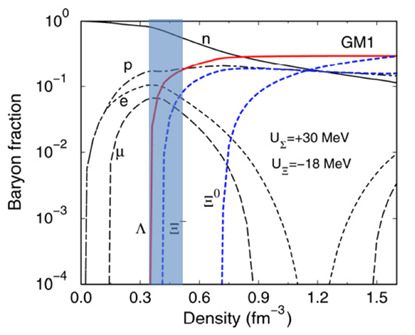
\includegraphics[width=90mm]{den_barion.png}
  \caption{密度に対する粒子の存在量\cite{MItudo}\label{fig:den_barion}}
\end{figure}
\begin{figure}[htbp]
  \centering
     
\includegraphics[width=120mm]{nodata.png}
\end{figure}
\newpage
\subsection{Double-$\Lambda$Hyper核}
通常の核に$\Lambda$粒子を2つ持たせたものがDouble-$\Lambda$Hyper核である。
Double-$\Lambda$Hyper核を生成するため、K$^+$,K$^-$反応により$\Xi$$^-$粒子を生成する。
K$^+$,K$^-$反応は式(\ref{eq:K+-})の反応である。
そして、生成された$\Xi$$^-$粒子を原子核に吸収させることで式(\ref{eq:Xi_eq})の反応を起こし$\Lambda$粒子を生成する。
\begin{equation}
	\ce{K- + p -> $\Xi$- + K+}
\label{eq:K+-}
\end{equation}
\begin{equation}
	\ce{$\Xi$- + p -> $\Lambda$ + $\Lambda$ + 28.6Mev}
\label{eq:Xi_eq}
\end{equation}
\par
E07実験では、K$^-$粒子を生成しDiamond Targetに照射することで$\Xi$$^-$粒子を生成する。
そして、生成された$\Xi$$^-$粒子を原子核乾板中で静止させる。
$\Xi$$^-$粒子は電離損失により$\Xi$$^-$粒子の持つエネルギーが減少していく。
エネルギーが減少した後に乾板中の原子核に吸収されることで、核内の陽子と反応を起こす。
これらの反応により生成された2つの$\Lambda$粒子が原子核の中にとどまると、Single-$\Lambda$Hyper核やDouble-$\Lambda$Hyper核が生成される。
\par
E07実験では上述したとおり原子核乾板の外で$\Xi$$^-$粒子を生成し、乾板中で$\Xi$$^-$粒子を反応させる。
しかし、それ以外にもK$^-$粒子が原子核乾板の中の原子核と反応しDouble-$\Lambda$Hyper核ができる場合もある。
\par
\begin{figure}[htbp]
  \centering
     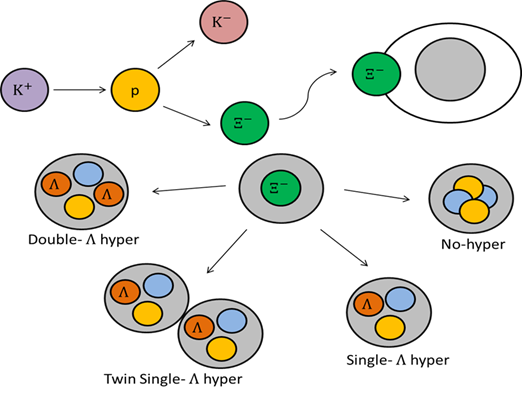
\includegraphics[width=120mm]{makehyper.png}
  \caption{Hyper核生成過程\label{fig:makehyper}}
\end{figure}
\newpage
\subsection{原子核乾板}
原子核乾板とは非常に高感度な写真フィルムの一種で、荷電粒子の通過した跡を記録する検出器である。
私たちが実験で使用する$\Lambda$粒子の寿命は非常に短いため、Hyper核の生成・崩壊事象をすべて記録できる原子核乾板を使う必要がある。
\par
原子核乾板はBaseと呼ばれるポリスチレンフィルムで作成された支持体にEmulsionを塗布して作成している。
Emulsionは通常の写真乳剤よりもハロゲン化銀の含有量が高く,最小電離損失に対して感度を持っているものである。
E07実験で使用する原子核乾板1400枚(薄型:200、厚形:1200)はすべて岐阜大学で製造された。
\par
E07実験で使用する乾板は40 $\mu$mのBaseに450 $\mu$mの乳剤を塗布する厚型乾板と、180 $\mu$mのBaseに100 $\mu$mの乳剤を塗布する薄型乾板の二種類である。
\par
薄型乾板はSSDとemulsionとの接続に使用される。
薄型乾板はbaseが厚く、乳剤が薄く塗布されているため現像の前後で乾板の変形が小さい。
そのため、記録された飛跡の角度や位置を明確に求められる。
\par
厚形乾板は照射された$\Xi$粒子を乾板中で静止させ、娘粒子の飛跡を記録するために用いられる。
そのため、荷電粒子飛跡が記録されないbaseを薄くし、乳剤の塗布量を多くすることでハイパー核事象の全飛跡を乾板中で記録する。
\par
\begin{figure}[htbp]
  \centering
     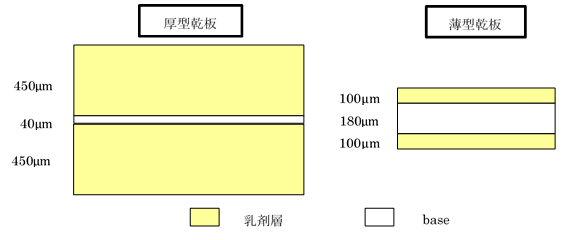
\includegraphics[width=140mm]{emulsionorder.png}
  \caption{使用する原子核乾板の規格\label{fig:emulsionorder}}
\end{figure}
\par
\newpage
原子核乾板の利点としては大きく分けて2点ある。
\par
一点目は、現像処理を行うことで半永久的に顕微鏡による観測を可能にすることである。
原子核乾板中を荷電粒子が通ることで、原子核乾板の主成分であるAgBrが電離され銀原子が生成される。(図\ref{fig:process_recored_track}(a))
現像処理により、銀が成長し1$\mu$m程度の粒となり(grain)、荷電粒子の飛跡がgrainの連なり(track)として現れ、その状態を保持する。(図\ref{fig:process_recored_track}(b))
そのため、原子核乾板を破損しない限り一度記録したHyper核の生成・崩壊事象やHyper核以外の荷電粒子秘跡を何度でも同じ状態で観測することができる。
\par
二点目は、サブミクロン精度での空間分解能を持つことである。
生成される銀粒子の大きさが$\mu$mオーダーのため、その大きさでの位置分解能が出る。
また、乾板に記録された飛跡の長さ、太さは通過した荷電粒子のエネルギーや電荷に依存する。
そのため、私たちは記録されたHyper核事象の飛跡の長さと角度からエネルギーを計算することで$\Lambda$-$\Lambda$間に働く相互作用を算出することができる。
\begin{figure}[htbp]
  \centering
      \begin{tabular}{c}
        % 1枚目の画像
        \begin{minipage}{0.5\hsize}
          \centering
            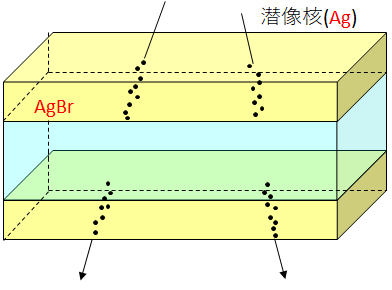
\includegraphics[clip, width=60mm]{process_bdev.png}
            \hspace{1.6cm} (a)現像前
        \end{minipage}
        
        % 2枚目の画像
        \begin{minipage}{0.5\hsize}
          \centering
            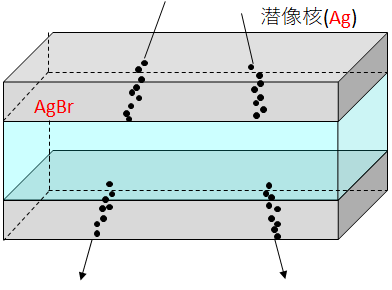
\includegraphics[clip, width=60mm]{process_adev.png}
            \hspace{1.6cm} (b)現像後
        \end{minipage}
    
      \end{tabular}
      \caption{原子核乾板中に飛跡が記録される過程の模式図\label{fig:process_recored_track}}
\end{figure}
\begin{figure}[htbp]
 \centering
      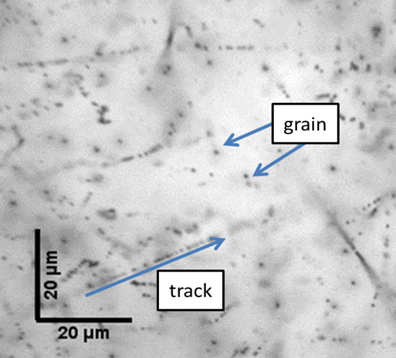
\includegraphics[width=70mm]{grainfog.png}
 \caption{原子核乾板中に記録されるtrackとgrain\label{fig:grain_track}}
\end{figure}
\subsection{光学顕微鏡}
光学顕微鏡を用いて、現像後の原子核乾板に記録されているtrackを追跡、観察する。
使用する顕微鏡は、モーターによって水平方向(x、y方向)に約1 $\mu$mの精度で位置制御し、
エンコーダーによって鉛直方向(z方向)に約0.1 $\mu$mの精度で稼働できる。
この顕微鏡により、原子核乾板表面の推測される位置で目的のtrackを探し、$\Xi$$^-$粒子候補を見つけ、trackを原子核乾板上面から下面まで追跡していく。
\par
PCを接続することで、この光学顕微鏡を制御している。
CCDカメラを顕微鏡に設置することで、顕微鏡で観察したものを画像として取得する。
取得した画像をPCの画面上に表示することや、顕微鏡の稼働に活用している。
$\Xi$$^-$粒子自動追跡には、50倍の対物レンズを使用している。
\begin{figure}[htbp]
  \centering
     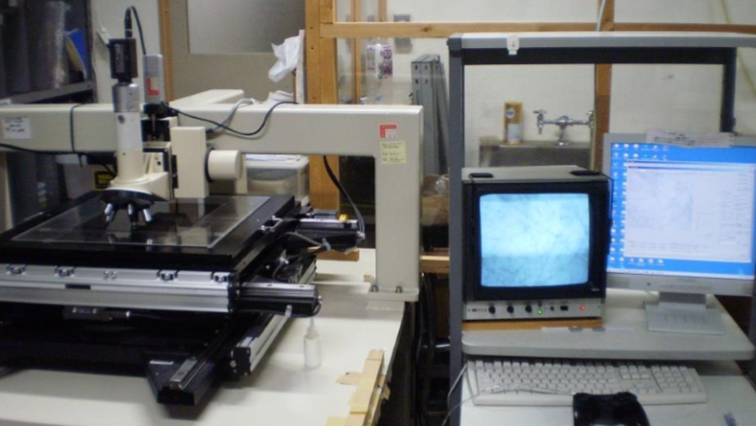
\includegraphics[width=140mm]{microscope.png}
  \caption{光学顕微鏡\label{fig:microscope}}
\end{figure}
\newpage
\subsection{KEK-PS E373実験}
E373実験はE176実験に続くDouble-$\Lambda$Hyper核検出実験である。
\cite{Nagara}
\cite{Nagara2}
E176実験の約10倍のDouble-$\Lambda$Hyper核の検出を目標にし、エマルジョンとカウンターを組み合わせたハイブリッド-エマルジョン法を取り入れて実施された。
約1000の$\Xi$$^-$粒子吸収事象が見積もられ、光学顕微鏡を用いた半自動飛跡追跡により全モジュールの解析が終了している。
解析の結果、ハイブリッド-エマルジョン法により約600例の$\Xi$$^-$粒子吸収事象を検出し、7例のDouble-$\Lambda$Hyper核を検出した。
その中でも、“NAGARA Event”と名付けられた事象は、Double-$\Lambda$Hyper核の生成・崩壊過程を一意に決定することができた。(図\ref{fig:Nagara})
これにより、$\Lambda$-$\Lambda$間相互作用エネルギー(\ce{$\Delta$B_{$\Lambda$$\Lambda$}} = 0.67 $\pm$ 0.17 MeV)および
$\Lambda$粒子の核内での結合エネルギー(\ce{B_{$\Lambda$$\Lambda$}} = 6.91 $\pm$ 0.16 MeV)から$\Lambda$-$\Lambda$間相互作用が
弱い引力であることを示した。\cite{Nagara}
\par
また、原子核乾板のすべてを撮影しハイパー核事象を検出する全面探査法を開発する中でツインハイパー核を検出し、“Kiso Event”と名付けた。
(図\ref{fig:Kiso})
これまで$\Xi$$^-$粒子が束縛される原子軌道はほとんどが3D軌道と言われていたが、
この事象により$\Xi$$^-$粒子が束縛される原子軌道は3D軌道より深く束縛されることを示した。\cite{Kiso}
\par
現在のストレンジネス核物理に関する確かな実験データは“NAGARA Event”と“Kiso Event”のみである。
そのため、より多くのハイパー核事象の統計を必要とする。
\begin{figure}[htbp]
  \centering
      \begin{tabular}{c}
        % 1枚目の画像
        \begin{minipage}{0.5\hsize}
          \centering
            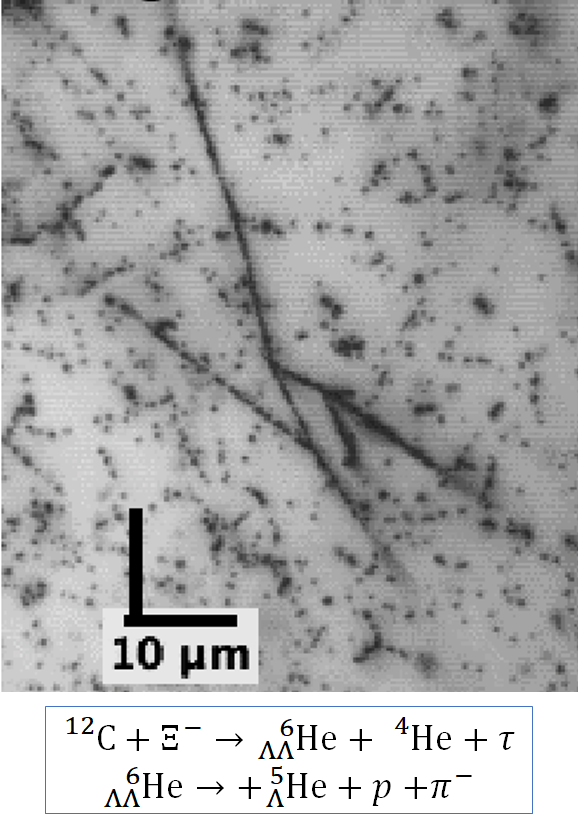
\includegraphics[clip, width=60mm]{Nagara_witheq.png}
            \hspace{1.6cm} 
            \caption{Nagara event\label{fig:Nagara}}
        \end{minipage}
        
        % 2枚目の画像
        \begin{minipage}{0.5\hsize}
          \centering
            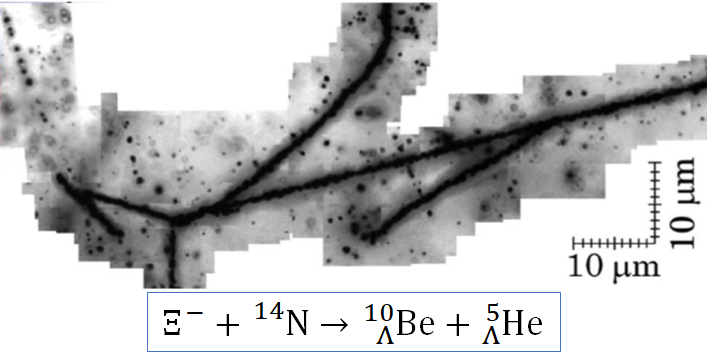
\includegraphics[clip, width=70mm]{Kiso_witheq.png}
            \hspace{1.6cm} 
            \caption{Kiso event\label{fig:Kiso}}
        \end{minipage}
    
      \end{tabular}
\end{figure}
\subsection{J-PARC E07実験}
J-PARC E07実験はハイブリッド-エマルジョン法によりKEK-PS E373実験の10倍の統計量を目指す実験である。
表\ref{tab:compare_E07_E373}はJ-PARC E07実験とKEK-PS E373実験の比較をしたものである。
表にあるように、beamのK$^-$/$\pi$$^-$を約3.5倍、原子核乳剤の量を約3倍にすることで10倍の$\Xi$$^-$粒子静止事象を実現する。
\begin{table}[htbp]
  \centering
  \caption{J-PARC E07実験とKEK-PS E373実験の比較\label{tab:compare_E07_E373}}
  \begin{tabular}{c|c|c}
     &KEK-PS E373実験&J-PARC E07実験\\
  \hline
  \hline
  $\Xi$$^-$粒子静止事象 & ~10$^3$    & ~10$^4$  \\
  K$^-$/$\pi$$^-$ & 1/4  & 6/1 \\
  原子核乳剤量 & 0.8t & 2.1t  \\
  \hline
  \end{tabular}
\end{table}
\par
図\ref{fig:e07setup}はE07実験のセットアップを示している。
1.8 GeV/cのK$^-$beamをダイアモンド標的に照射し、$\Xi$$^-$粒子を生成する。
E07実験では、原子核乾板の上流と下流にSSD(Silicon Strip Detector)を設置している。
SSDは電荷をもった粒子が通過した際に、通過した粒子が原子核乾板スタックのどの位置にどのような角度で照射されているかの情報を記録する検出器である。
SSDは4層構造になっているため、同タイミングで4層に渡って検出された座標情報を使い、通過した荷電粒子の角度を推定することができる。
原子核乾板スタックを2つのSSDで挟むことで、原子核乾板に照射された荷電粒子の位置情報、角度情報を記録する。
SSDに記録された情報を使い、
emulsionに記録された飛跡の中で$\Xi$$^-$粒子である確率の高い飛跡のみを追跡することでいち早くDouble-$\Lambda$Hyper核を検出する。
\begin{figure}[htbp]
  \centering
     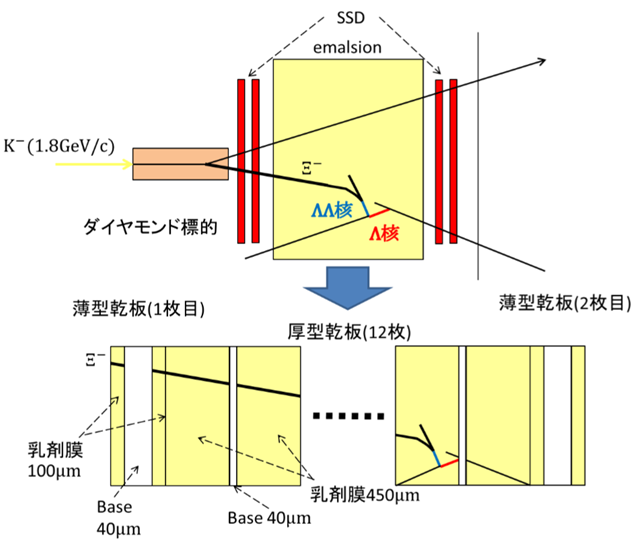
\includegraphics[width=95mm]{e07setup.png}
  \caption{E07実験のセットアップ\label{fig:e07setup}}
\end{figure}


\newpage
\section{J-PARC E07実験2nd Run}
J-PARC E07実験は1st Runを2016年6月18日〜30日に、2nd Runを2017年5月~7月に実施した。
1st Runでは18stacks、2nd Runでは100stacksのbeam照射に成功した。
beam照射を行うにあたり使用する原子核乾板のバックグラウンド削減法の実施、原子核乾板の真空パック法の確立、現像等を実施した。
\par
本章ではJ-PARC E07実験beam照射、現像においての実施内容及びその手法を述べる。
強制現像退行処理と原子核乾板の現像に関する詳細な情報及び処理の評価は大橋修士論文に記載する。
\subsection{Refresh処理の実施}
\subsubsection{実施背景}
J-PARC E07実験で使用する原子核乾板約1400枚はすべて岐阜大学ダブルハイパー核実験棟にて制作した。
制作は2013年12月~2014年3月の期間で完了している。
当初の予定では乾板製造後すぐにbeam照射を実施する予定であったが、J-PARCでの放射能漏れ事故により実験は延期になった。
\par
製造した原子核乾板は現像されるまで空気中の宇宙線やコンプトン電子等の荷電粒子を記録していく。
図\ref{fig:compton_and_cosmicray_in_emulsion}は原子核乾板中に記録されたコンプトン電子と宇宙線を示している。
これらのgrainや飛跡がバックグラウンドとして増加すると、beam照射後の解析に支障を来す恐れがある。
そこで、宇宙線の影響が少ない神岡鉱山内に鉛ブロックで箱を作り、製造した原子核乾板を保管した。(図\ref{fig:emulsion_in_Kamioka})
\begin{figure}[htbp]
  \centering
      \begin{tabular}{c}
        % 1枚目の画像
        \begin{minipage}{0.5\hsize}
          \centering
            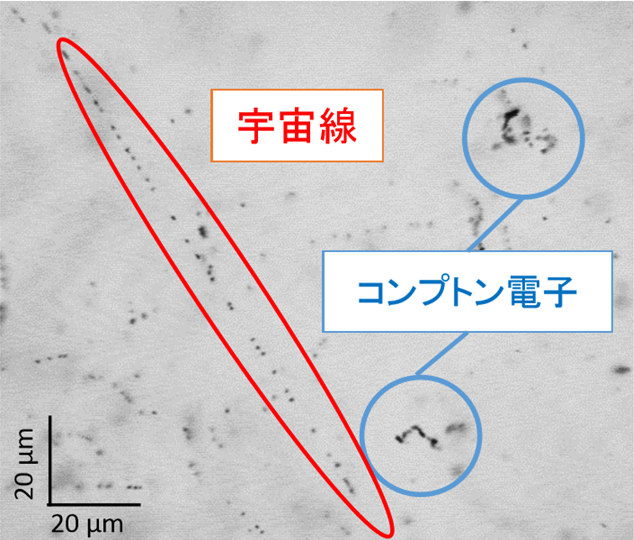
\includegraphics[clip, width=70mm]{compton_cosmiclay.png}
            \hspace{1.6cm} 
            \caption{乾板に記録されたコンプトン電子と宇宙線の飛跡\label{fig:compton_and_cosmicray_in_emulsion}}
        \end{minipage}
        
        % 2枚目の画像
        \begin{minipage}{0.5\hsize}
          \centering
            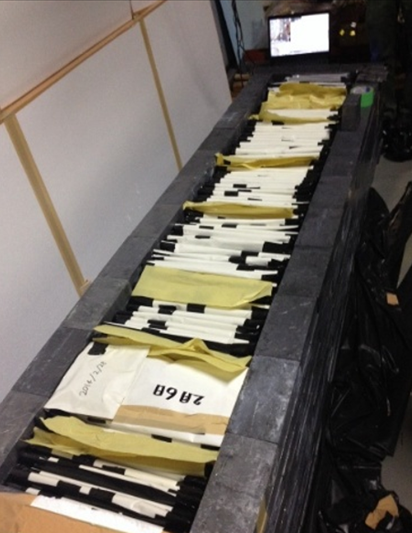
\includegraphics[clip, width=50mm]{emulsion_in_Kamioka.png}
            \hspace{1.6cm} 
            \caption{神岡鉱山内の鉛ブロック中に原子核乾板の保管状況\label{fig:emulsion_in_Kamioka}}
        \end{minipage}
      \end{tabular}
\end{figure}
\newpage
\par
図\ref{fig:stragecompton}は製造からの時間経過による原子核乾板記録された宇宙線、コンプトン電子の増加傾向を示している。
赤色が岐阜大学の冷蔵庫内で保管した場合、青色が神岡鉱山鉛箱内で保管した場合である。
二つの線の傾きを比較すると、神岡鉱山内で保管したことで非常に多くのバックグラウンドを削減することができたということが分かる。
\par
しかし、製造からbeam照射まで2年の期間が経過したため、神岡鉱山内で保管していたとしても解析に支障を及ぼすレベルまでバックグラウンドが蓄積してしまった。
制作から約2年間経過した原子核乾板には期間中神岡鉱山内で保管した場合、バックグラウンドが約130 event/10$^6$ $\mu$m$^3$となる。
図\ref{fig:beam_efficiency_to_compton}はコンプトンの蓄積量に対するbeam検出効率を示したものである。
図から2017年4月ごろにはバックグラウンドの蓄積によりbeam検出効率が50%にまで低下することが分かる。
そのため、蓄積されたバックグラウンドの消去のために原子核乾板に対して強制潜像退行処理(Refresh処理)を実施した。
\begin{figure}[htbp]
  \centering
     
\includegraphics[width=120mm]{nodata.png}
\end{figure}
\begin{figure}[htbp]
  \centering
     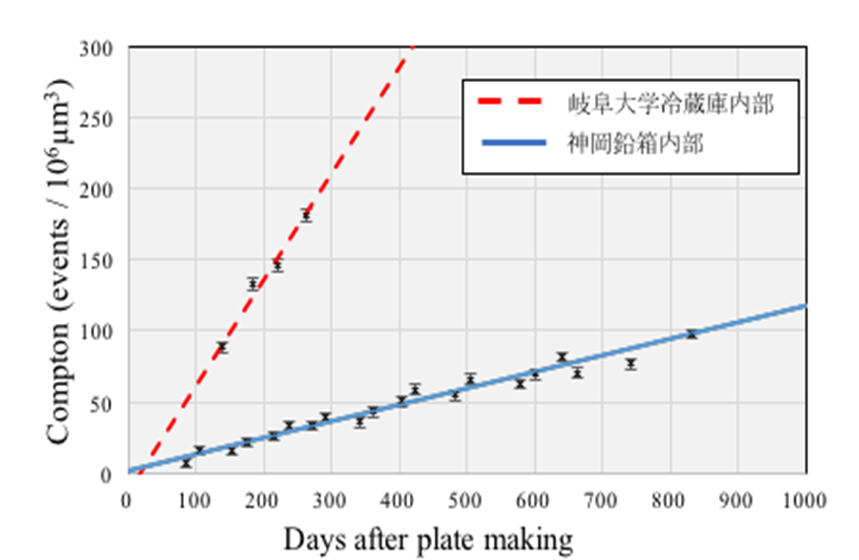
\includegraphics[width=120mm]{compton_strage.png}
  \caption{保管地点によるコンプトンの蓄積量\label{fig:stragecompton}}
\end{figure}
\begin{figure}[htbp]
  \centering
     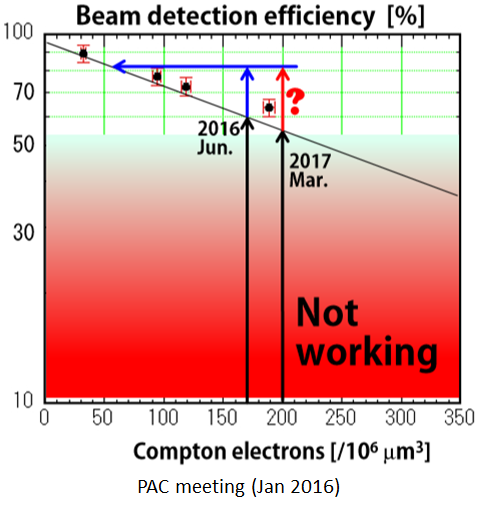
\includegraphics[width=90mm]{beam_efficiency_to_compton.png}
  \caption{コンプトンの蓄積量に対するbeamの検出効率\label{fig:beam_efficiency_to_compton}}
\end{figure}


\newpage
\subsubsection{原理}
写真フィルムには撮影してから現像するまでに時間を経ると、映像が消えていく性質(潜像退行性)がある。[式(\ref{eq:gennzou})]
 また、潜像退行性は高温高湿度の環境で著しく進むことが明らかになっている。
\begin{equation}
    \ce{Ag4 + O2 + 2H2O -> 4Ag+ + 4OH-}
\label{eq:gennzou}
\end{equation}
\par
原子核乾板は塗布されてから現像されるまでの間に、自然放射線や宇宙線の影響を受け潜像が蓄積される。
そこで、蓄積された潜像を消去するための手法として強制潜像退行処理(Refresh処理)と呼ばれる方法が開発されている。
\cite{takusann}
 Refresh処理は原子核乾板の持つ現像退行性を利用する。
図\ref{fig:intr_refresh}はRefresh処理の模式図である。
原子核乾板には荷電粒子が通過した跡に対して潜像核が形成されている。(図\ref{fig:intr_refresh}(a))
 原子核乾板中に記録された潜像核に対して式\ref{eq:gennzou}の反応を起こすことで、形成されていた潜像核がイオンになり現像されない状態になる。
(図\ref{fig:intr_refresh}(b))
 この化学反応は温度が高くなるほど反応が促進されるため、原子核乾板を高温高湿度の環境下に置くことで潜像退行が促進される。
よって、Refresh処理によりbeam照射の前に記録されたBackgroundを消去できる。(図\ref{fig:intr_refresh}(c))
\begin{figure}[htbp]
  \centering
      \begin{tabular}{c}
        % 1枚目の画像
        \begin{minipage}{0.33\hsize}
          \centering
            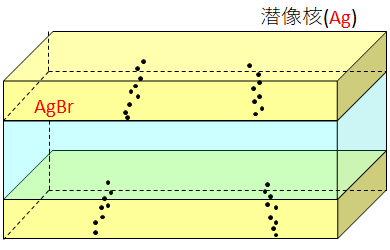
\includegraphics[clip, width=50mm]{ref_pro1.png}
            \hspace{1.6cm} (a)Refresh処理前
        \end{minipage}
        
        % 2枚目の画像
        \begin{minipage}{0.33\hsize}
          \centering
            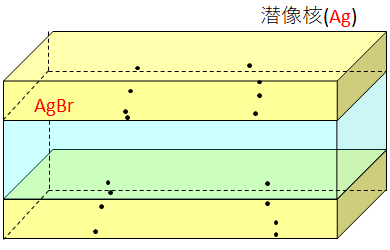
\includegraphics[clip, width=50mm]{ref_pro2.png}
            \hspace{1.6cm} (b)Refresh処理後
        \end{minipage}

        % 3枚目の画像
        \begin{minipage}{0.33\hsize}
          \centering
            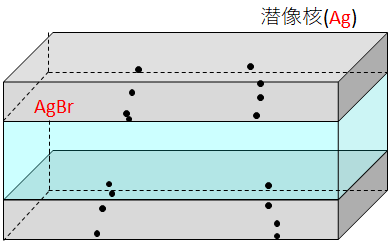
\includegraphics[clip, width=50mm]{ref_pro3.png}
            \hspace{1.6cm} (c)現像後
        \end{minipage}
    
      \end{tabular}
      \caption{Refresh処理模式図\label{fig:intr_refresh}}
\end{figure}
\subsubsection{実施環境}
E07実験で使用する原子核乾板に対してRefresh処理を実施場合は温度25度、湿度90%の環境を維持することが必要である。\cite{oohashi}
そこで、温度と湿度をコントロールするチェンバーを作成した。(図\ref{fig:refresh_masi-nn})
 このチェンバーは1度の処理で100枚の原子核乾板のRefresh処理を実施可能である。
図\ref{fig:refresh_hanga__}に示した乾板ハンガーを使用し、2枚一組の状態にして原子核乾板をチェンバーの中に入れた。
1st Runではこの装置を使い4回のRefresh処理を実施し、温度湿度の制御を手動で行った。
2nd Runでは13回のRefresh処理を、温度・湿度の調整を自動制御で実施した。\cite{muramoto}
\begin{figure}[htbp]
  \centering
     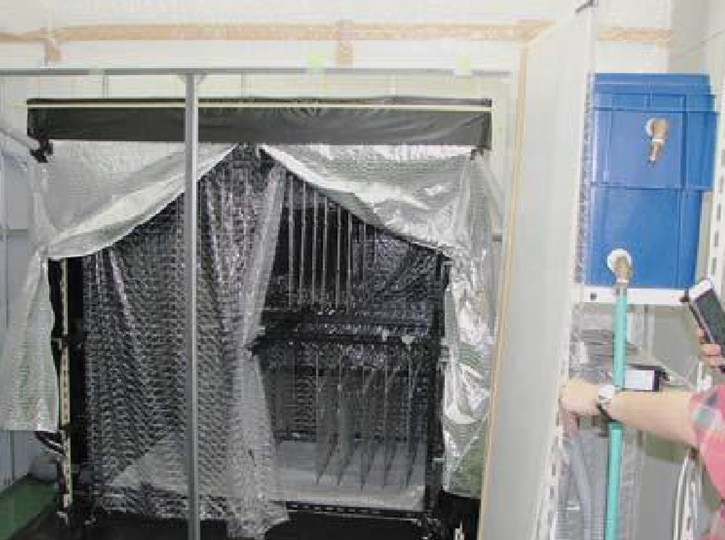
\includegraphics[width=140mm]{refresh_chember.png}
  \caption{Refreshチェンバー\label{fig:refresh_masi-nn}}
\end{figure}
\begin{figure}[htbp]
  \centering
     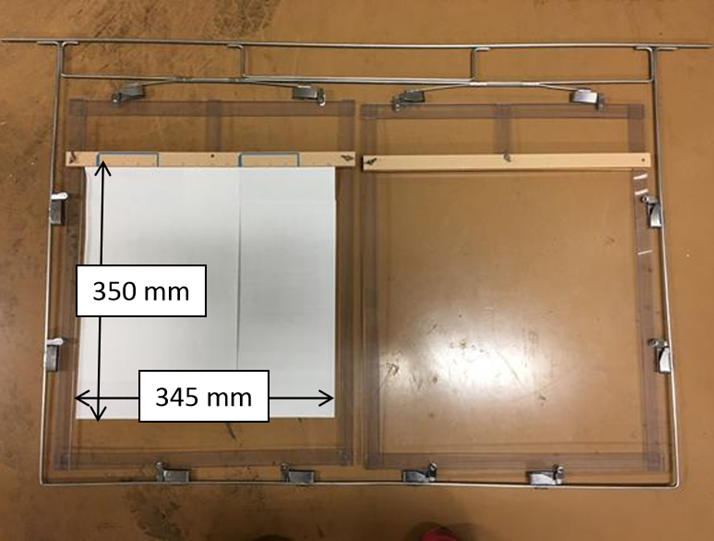
\includegraphics[width=100mm]{refresh_hanga.png}
  \caption{乾板ハンガー\label{fig:refresh_hanga__}}
\end{figure}
\subsection{GridMark照射環境の最適化}
\subsubsection{暗室の拡張}
1st Runではbeam照射後の原子核乾板を岐阜に持ち帰り、現像の数日前に岐阜でGridマークを照射した。
beam照射からGridマーク照射までの間に乾板の変形があったせいか、Gridマークの位置ズレが一様でなかったため一視野内に飛跡を持ってくることが困難になった。
1st Runの結果から、2nd Runではbeam照射後の原子核乾板に対してJ-PARC内の暗室下でGridMark照射を実施した。
そのためGridMark照射装置を設置するためE07実験1st Run時に設置した暗室の拡張を行った。
\par
図\ref{fig:darkroom_mosikizu}、\ref{fig:darkroom_view}は暗室拡張後を示したものである。
横の長さを1m拡張することで、Gridマーク照射装置を設置する場所を確保した。
\begin{figure}[htbp]
  \centering
    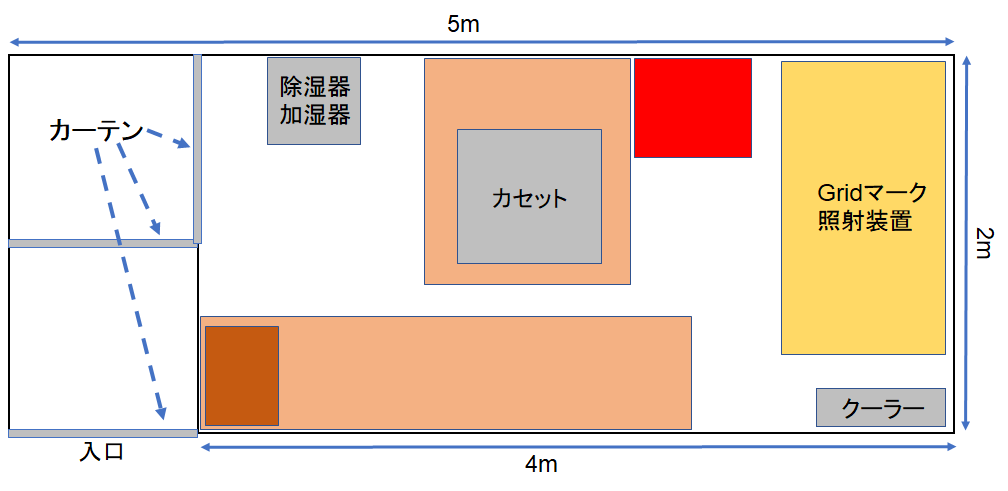
\includegraphics[width=120mm]{darkroom_after.png}
  \caption{拡張後暗室内図\label{fig:darkroom_mosikizu}}
\end{figure}
\begin{figure}[htbp]
  \centering
    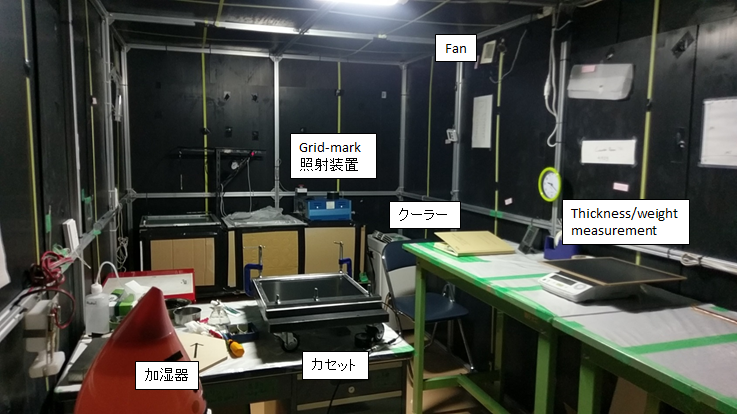
\includegraphics[width=120mm]{darkroom_view.png}
  \caption{暗室内部\label{fig:darkroom_view}}
\end{figure}
\newpage
\par
暗室拡張後、暗室内が原子核乾板を取り扱うのに適した環境であるかどうかを確認した。
暗室内湿度は加湿器・除湿器を設定し常時50%を超えるように設定した。
室温はクーラーにより常時20-25℃になるように設定した。
図\ref{fig:darkroom_onndo}、\ref{fig:darkroom_situdo}は暗室拡張後、暗室内の温度・湿度を約5時間モニターした結果である。
図\ref{fig:darkroom_onndo}、\ref{fig:darkroom_situdo}より、
暗室内は温度・湿度が一定に保たれており、原子核乾板を取り扱うのに適した環境にできていると判断をしたうえで、
原子核乾板の取り扱いを行った。
\begin{figure}[htbp]
  \centering
    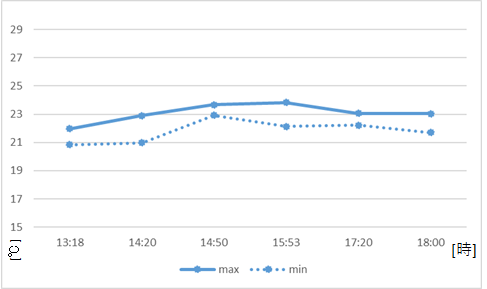
\includegraphics[width=120mm]{darkroom_temp.png}
  \caption{暗室内の温度\label{fig:darkroom_onndo}}
\end{figure}
\begin{figure}[htbp]
  \centering
    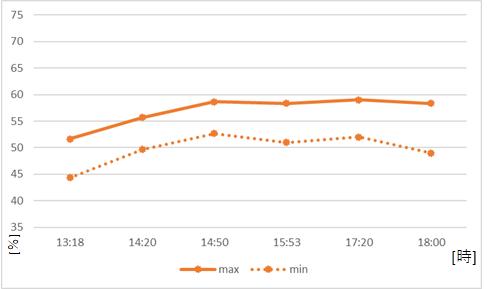
\includegraphics[width=120mm]{darkroom_mist.png}
  \caption{暗室内の湿度\label{fig:darkroom_situdo}}
\end{figure}
\subsubsection{GridMarkネガ}
2016年にE07実験testRunとしてbeam照射を実施した。
その際、原子核乾板に焼き付けたGridマークの中にはネガのつまりにより、Gridマークが照射されていないものが存在していた。
1st RunのGridマーク照射の際はネガのつまり部分に対して空気を送り、ネガの穴に詰まった乾板の破片を除去しながら照射を行った。
しかし、1st Runの原子核乾板においてもGridマークが照射されていない箇所が存在した。
これらを受けてネガの変更を行った。
2nd Runでは銅と真鍮板の加工を株式会社 ナノプロセス様に依頼し、加工と原子核乾板に対する影響を考慮してネガの素材を銅に決定した。
E07実験2nd Runの原子核乾板には図\ref{fig:nega_2ndRun}を使いGridマークを照射した。
\begin{figure}[htbp]
  \centering
    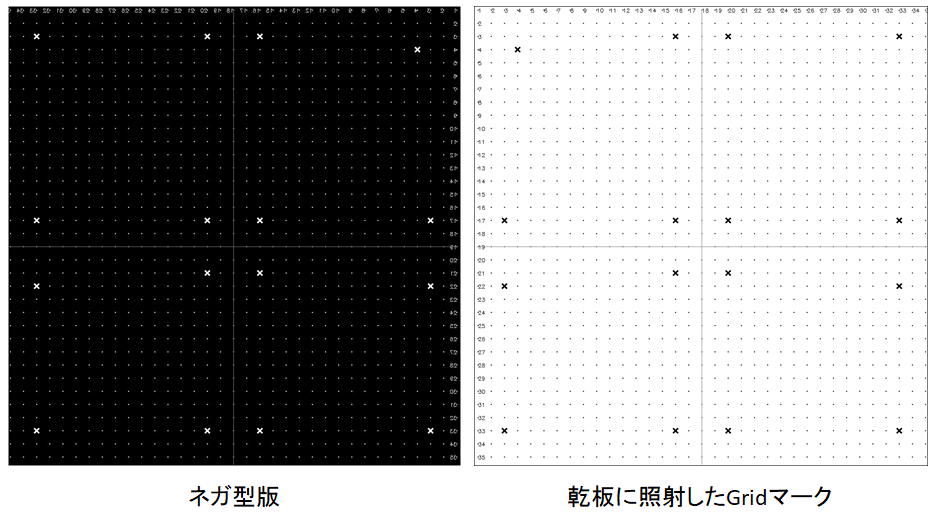
\includegraphics[width=140mm]{grid_nega2.png}
  \caption{E07実験2ndRunネガ\label{fig:nega_2ndRun}}
\end{figure}
\newpage
\subsubsection{GridMark照射装置}
E071st Runではタイマーを用いて10秒間原子核乾板に露光した。
図\ref{fig:grid_1stRun}は1stRunのGridマーク照射の模式図である。
1st Runは先行研究と同様の方法を用いて照射をした。\cite{tamura}
Gridマーク照射装置の操作者がストロボ装置のスイッチを入れると同時にストップウォッチのスイッチを入れる。
ストップウォッチで10秒間露光した後ストロボ装置の電源を切り、Gridマーク照射を終了する。
この先行研究と同様の手法では1mod分照射するのに約1時間半の時間が必要になる。
E07実験2nd Runではbeam照射後すぐにGridマークを照射する。
従来の手法から変更することで照射の時間短縮及び疲労の削減のために照射装置の改造を行った。
\begin{figure}[htbp]
  \centering
     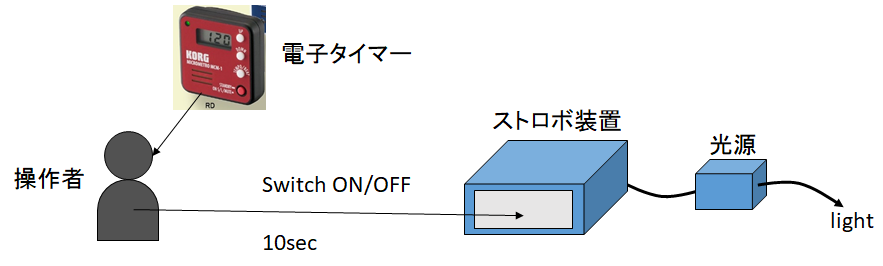
\includegraphics[width=120mm]{grid_1stRun.png}
  \caption{1st RunGridマーク照射模式図\label{fig:grid_1stRun}}
\end{figure}
\begin{figure}[htbp]
  \centering
     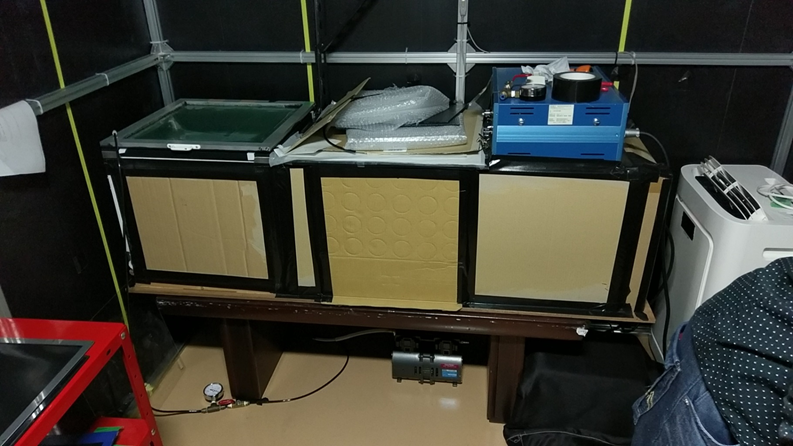
\includegraphics[width=120mm]{grid_printer.png}
  \caption{Gridマーク照射装置\label{fig:grid_masi-nn}}
\end{figure}
\newpage
\par
2nd RunのGridマーク照射ではストロボスタートボタンを設け、指定の回数発行した後自動でストロボのスイッチを切るように設定した。
1st Runで運用したストロボ光照射条件は、点滅周期1024 rpmで動作時間10秒だった。\cite{tamura}
1024 rpmは17.07 Hz(T=58.6msec.)のため発光回数は約171回。
したがってストロボスタートボタンの挙動は100Hz*1.71秒(10msec*171回)とした。
\par
2nd RunのGridマーク照射は図\ref{fig:grid_botan}を押すことで高速での照射を可能にした。
\begin{figure}[htbp]
  \centering
     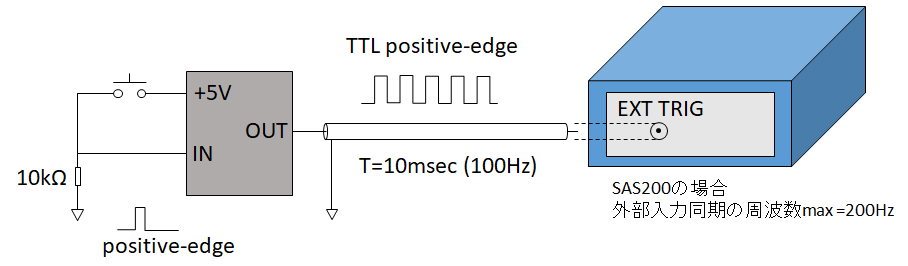
\includegraphics[width=120mm]{grid_kairo.png}
  \caption{Gridマークトリガー回路\label{fig:grid_kairo}}
\end{figure}
\begin{figure}[htbp]
  \centering
     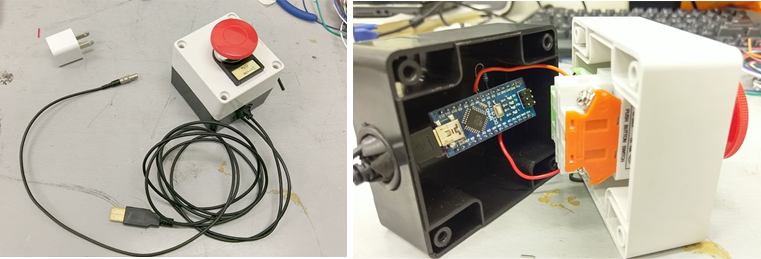
\includegraphics[width=120mm]{grid_botan.png}
  \caption{Gridマークトリガーボタン\label{fig:grid_botan}}
\end{figure}
\newpage
\subsection{E07実験2nd Runbeam照射}
\subsubsection{作業内容}
2017年5月~7月にかけて100stacksの原子核乾板すべてにbeam照射を行った。
原子核乾板にbeam照射を実施するために、温度、湿度が調整された暗室内で原子核乾板をEmulsion Casetteに詰め、
カセット内部の真空度を調節することが必要になる。
暗室内で原子核乾板をEmulsion Casetteに詰める際の流れは以下の通りである。
この作業は、先行研究で確立した方法に基づいて実施した。\cite{endo}
\begin{enumerate}
    \item beam照射8時間前に乾板を冷蔵庫から出し、常温に慣らしておく。
    \item グリスを塗った、Oリングをはめ込む。
    \item カセットの4つ角にL字のSUS板を置く。 
    \item 袋から乾板を開けて乾板の重さ・厚さを測定し、乾板の番号を記録、乾板にMOD番号を書く。
    \item 乾板をL字のSUS板に沿って原子核乾板13枚をカセットに入れる。
    \item 1.0 mm厚のSUS枠のゴム板側にシリコングリスを塗り、SUS枠をはめる。(図\ref{fig:tezyun_6})
    \item 1.0 mm厚のゴム板をはめる。(図\ref{fig:tezyun_7})
    \item 木の板を置き,その上におもりを置くことで乾板を固定した後,L字のSUS板を外す。(図\ref{fig:tezyun_8})
    \item カセットおさえを置き,ねじを軽くしめる。(図\ref{fig:tezyun_9})
    \item ねじを数回に分けてしめる。
    \item 図\ref{fig:ponpu}の水流真空ポンプで10分減圧し,1時間経過後もう一度減圧する。
\end{enumerate}
\begin{figure}[htbp]
  \centering
      \begin{tabular}{c}
        % 1枚目の画像
        \begin{minipage}{0.5\hsize}
          \centering
            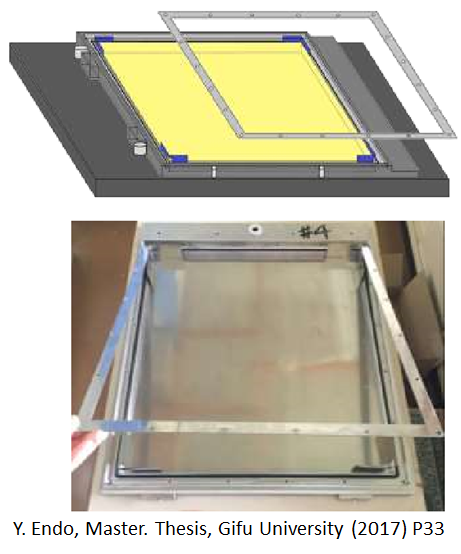
\includegraphics[clip, width=70mm]{tezyun_6.png}
            \hspace{1.6cm} 
            \caption{手順6\label{fig:tezyun_6}}
        \end{minipage}
        
        % 2枚目の画像
        \begin{minipage}{0.5\hsize}
          \centering
            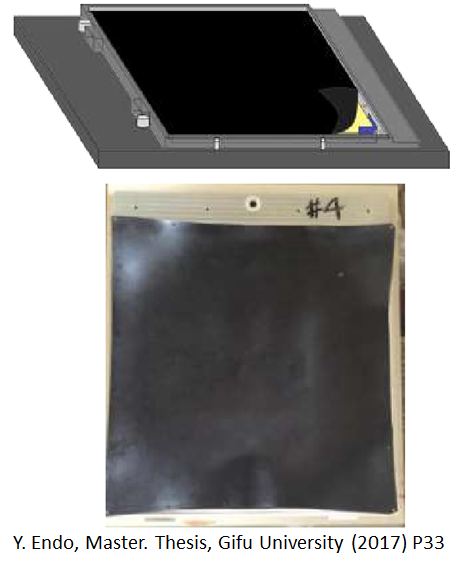
\includegraphics[clip, width=70mm]{tezyun_7.png}
            \hspace{1.6cm} 
            \caption{手順7\label{fig:tezyun_7}}
        \end{minipage}
    
      \end{tabular}
\end{figure}
\begin{figure}[htbp]
  \centering
      \begin{tabular}{c}
        % 1枚目の画像
        \begin{minipage}{0.5\hsize}
          \centering
            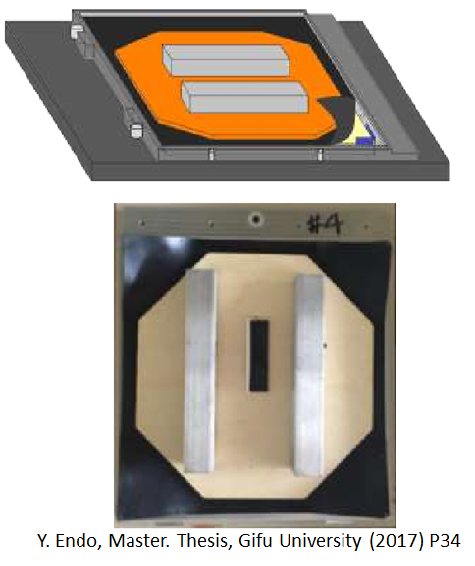
\includegraphics[clip, width=70mm]{tezyun_8.png}
            \hspace{1.6cm} 
            \caption{手順8\label{fig:tezyun_8}}
        \end{minipage}
        
        % 2枚目の画像
        \begin{minipage}{0.5\hsize}
          \centering
            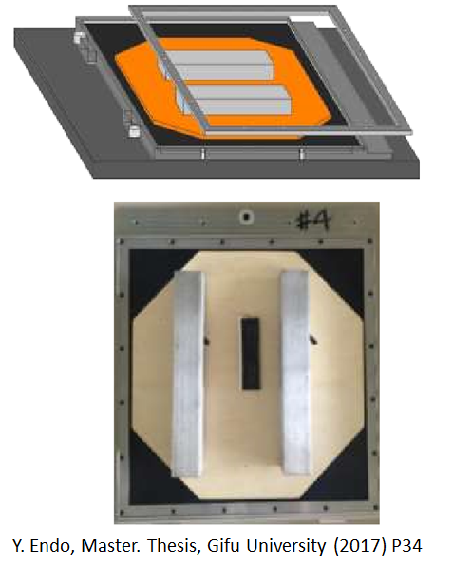
\includegraphics[clip, width=70mm]{tezyun_9.png}
            \hspace{1.6cm} 
            \caption{手順9\label{fig:tezyun_9}}
        \end{minipage}
    
      \end{tabular}
\end{figure}
\begin{figure}[htbp]
  \centering
    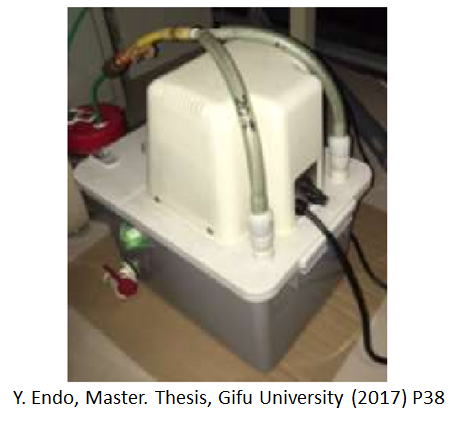
\includegraphics[width=70mm]{ponpu.png}
  \caption{水流ポンプ\label{fig:ponpu}}
\end{figure}
\newpage
\subsubsection{Emulsion Casetteでの真空度}
図\ref{fig:e07setup_real}はE07実験のbeamラインを示したものである。
私たちは暗室内にて1mod分の原子核乾板13枚(厚型:11枚、薄型2枚)をEmulsion Casetteに詰めてbeamラインにセットした。
図\ref{fig:e07setup_real}に示したEmulsion CasetteとSSDの間には5 mmしか距離がない。
そのため、Emulsion Casetteに原子核乾板を入れ、beam照射中に適切な真空度を保つことが必要である。
\begin{figure}[htbp]
  \centering
    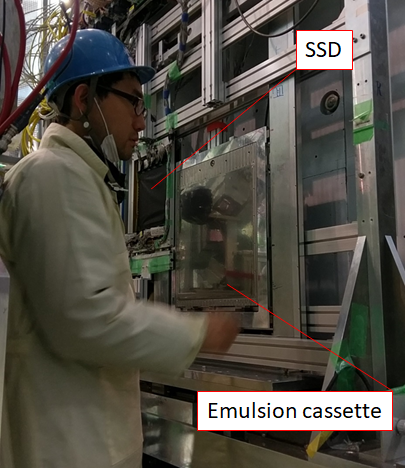
\includegraphics[width=70mm]{e07setup_real.png}
  \caption{E07beamライン\label{fig:e07setup_real}}
\end{figure}
\newpage
\par
私たちはbeamタイム中に4台のカセットを使用し、常にストックを持ち続けながらカセットを供給することができ、
beamタイムのロスを最小限にして実験を実施できた。
beam照射直前までパッキングしたカセットの内圧をモニターし続け、Mod$\#$19~Mod$\#$118の全真空度に問題が無いことを確認したうえで、
beamラインにカセットを提供した。
Mod$\#$19~Mod$\#$118のカセットの内圧の結果を付録に記載する。
例としてMod$\#$117のカセット内圧の変化を図\ref{fig:casette_bakyu-mu}に示す。
真空度の基準は『減圧後,内圧の変化が 10 時間経過しても 0.02 MPa 以下』と先行研究で定められた。\cite{endo}
E07実験2nd Runにおいても定められた真空度の基準をクリアしたEmulsion Casetteをbeamラインに提供した。
\begin{figure}[htbp]
  \centering
     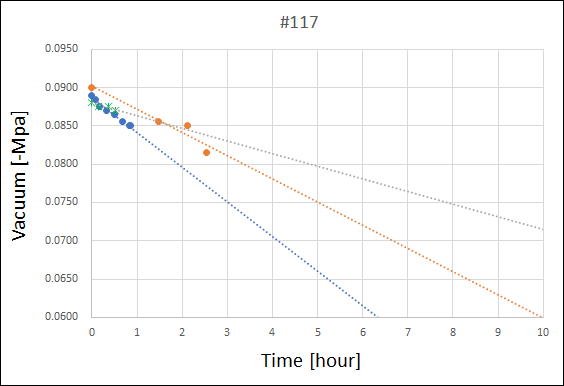
\includegraphics[width=140mm]{vacuum117.png}
  \caption{カセット内圧変化\label{fig:casette_bakyu-mu}}
\end{figure}
\newpage
\subsubsection{Emulsion Casetteの固定法確立}
1st Runのbeam照射ではカセットのSUS箔が18回の真空パックにより何度もはがれた。
2nd Runのbeam照射では100回の真空引きを行う必要があるため、この頻度でSUS箔が剥がれた場合対応しきれない。
そこで、カセットのSUS箔にかかる負荷軽減のための冶具が開発された。(図\ref{fig:casette_fix})
この治具を使用して、2nd Runの照射を行った。
これにより、2nd Runでは100回の真空引きに対して1度しかSUS箔が剥がれなかったため、全beam照射を通してカセットを提供することができた。
\begin{figure}[htbp]
  \centering
      \begin{tabular}{c}
        % 1枚目の画像
        \begin{minipage}{0.5\hsize}
          \centering
            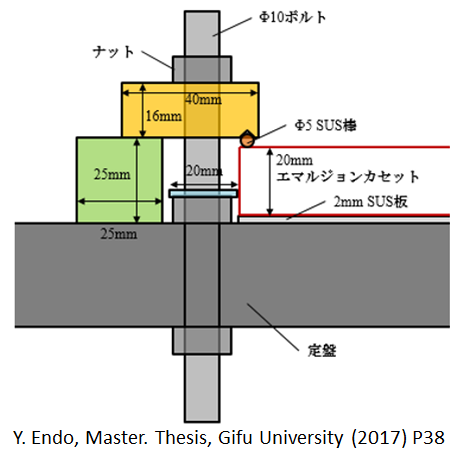
\includegraphics[clip, width=60mm]{casette_fix_moderu.png}
        \end{minipage}
        
        % 2枚目の画像
        \begin{minipage}{0.5\hsize}
          \centering
            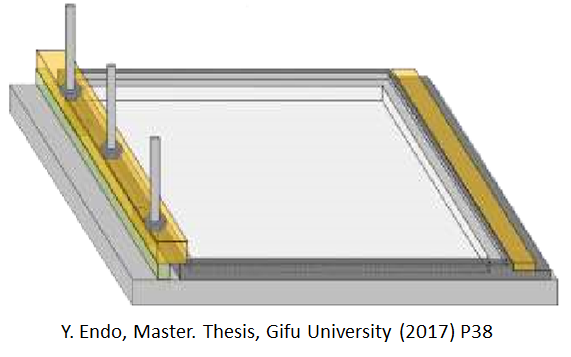
\includegraphics[clip, width=60mm]{casettefix.png}
        \end{minipage}
    
      \end{tabular}
      \caption{使用したカセット固定冶具の設計図\label{fig:casette_fix}}
\end{figure}
\newpage
\subsubsection{照射した乾板の密度}
2nd Runでは1st Runと同様にEmulsion Casetteに乾板を入れる前に乾板の厚さと重さの測定、
beam照射後に乾板の重さを測定することでbeam照射により乾板の重さに大きな変動がないかを確認した。
照射の前後で重さが1.0g以上異なっていた場合は、再度厚さ重さの測定をして記録した。
乾板の重さは電子天秤を用いて、乾板の厚さはシックネスゲージを用いて乾板の四つ角を測定した。
\par
1st Run乾板の密度はRefresh未処理の乾板、2nd RunはRefresh処理実施乾板での密度で図\ref{fig:hisuto}のようにヒストグラムを作成し、
ガウスフィッティングにより密度とその誤差を求めた。
フィッティングにより算出した1st Run乾板の密度の測定結果と2nd Run乾板の密度をまとめたものが表\ref{tab:compare_E07_12}である。
比較すると、1st Runと2nd Runで使用した原子核乾板に大きな違いは無いことが分かる。
また、図\ref{fig:kasozai}はE07実験で使用する原子核乾板を作成する際に使用した可塑剤の添加量に対する原子核乾板厚型の密度を示したものである。
この図と表の数値を比較すると、可塑剤の添加量に対応した密度になっていることが分かる。
このことから、Refresh処理の有無で原子核乾板の密度が変化せず、1st Runと2nd Runで使用した原子核乾板の密度に違いは無い。
\par
薄型乾板でも同様に密度の比較をした。
表\ref{tab:compare_E07_12}を見ると、1st Runの薄型乾板は厚形乾板より密度が大きく算出されていたが、2nd Runで使用した薄型乾板でも同様の傾向になった。
\begin{figure}[htbp]
  \centering
     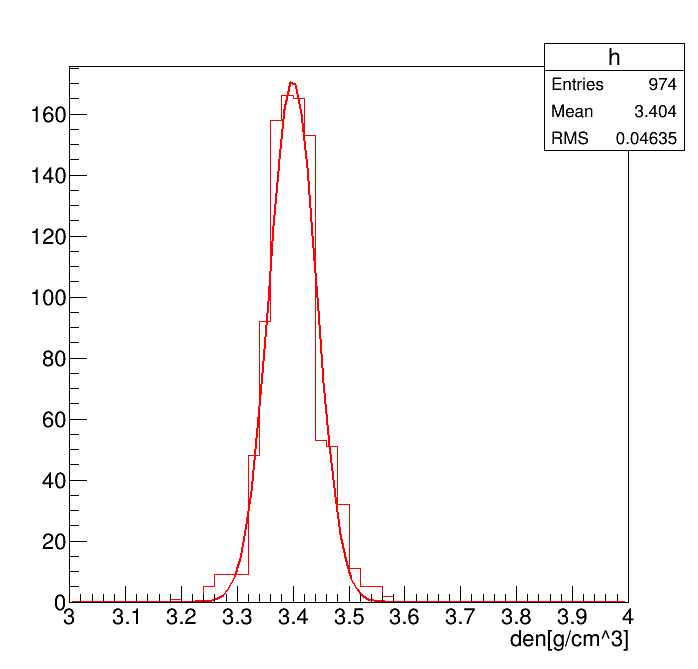
\includegraphics[width=70mm]{thick75_den.png}
  \caption{ヒストグラム\label{fig:hisuto}}
\end{figure}
\begin{table}[htbp]
  \centering
  \caption{J-PARC E07実験で使用した原子核乾板の密度\label{tab:compare_E07_12}}
  \begin{tabular}{c|c|c}
     &1st Run [g/cm$^3$]&2nd Run [g/cm$^3$]\\
  \hline
  \hline
  可塑剤6.0cc 厚型乾板 & 3.48 $\pm$ 0.04 & 3.43 $\pm$ 0.05 \\
  可塑剤7.5cc 厚型乾板 & 3.41 $\pm$ 0.07 & 3.40 $\pm$ 0.04 \\
  可塑剤7.5cc 薄型乾板 & 3.73 $\pm$ 0.16 & 3.74 $\pm$ 0.13 \\
  \hline
  \end{tabular}
\end{table}
\begin{figure}[htbp]
  \centering
     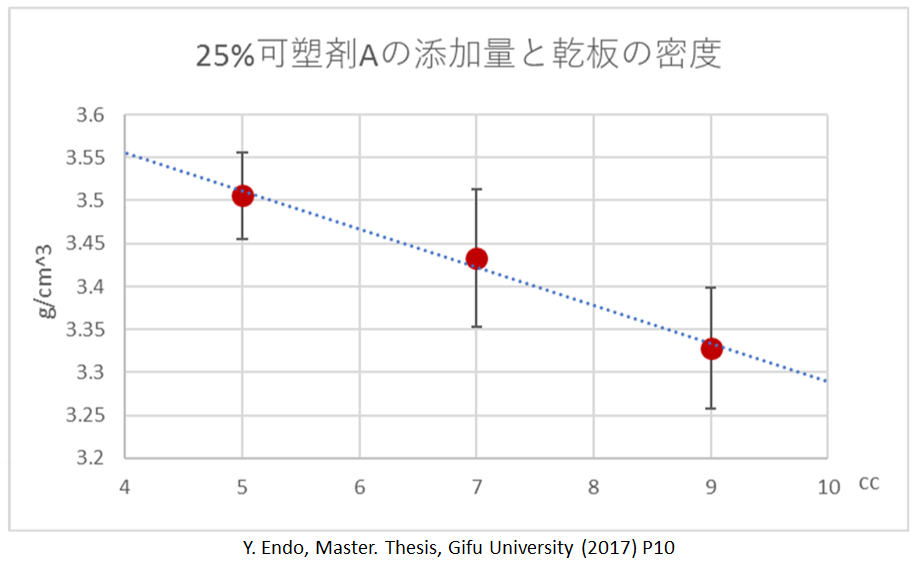
\includegraphics[width=140mm]{kasozai.png}
  \caption{可塑剤Aの添加量に対する原子核乾板の密度\label{fig:kasozai}}
\end{figure}
\newpage
\subsection{現像}
\subsubsection{原理}
原子核乾板の現像には予浸(presoark)、現像(Cold.dev Hot.dev)、現像(Cold.dev Hot.dev)、停止(Stop)、定着(Fix2/4、Fix4/4)、水洗(Wash)の工程がある。
原子核乾板はこの順で工程を実施することで、記録した荷電粒子飛跡を顕微鏡で観察できるようになる。
\par
予浸(presoark)とは、原子核乾板に水分を吸収させる工程である。
beam照射の際も原子核乾板は乾燥した状態で実施している。
乾燥した状態では、これ以降の工程で使用する現像液や薬品が浸透しにくくなり、現像のムラが発生する恐れがある。
そのため、現像液が原子核乾板の表面だけでなく内部にも浸透しやすくするために、乾燥した原子核乾板に水分を吸収させる。
\par
現像(Cold.dev Hot.dev)とは、原子核乾板中で荷電粒子により生成された銀粒子の形成を促進する工程である。
荷電粒子飛跡によって形成された銀粒子を選択的に現像したいため、原子核乾板の現像にはAmidolを使用する。
\par
停止(Stop)とは、現像の工程で促進された銀粒子の形成促進の反応を停止させる工程である。
現像では荷電粒子によって形成された銀粒子のみ選択的に形成促進させている。
しかし、原子核乾板中には大量の銀粒子が存在しているため、銀粒子の形成促進を行いすぎるとすべての銀粒子が現像されてしまう。
我々は荷電粒子によって形成された銀粒子のみを観察する必要があるため、停止の工程で現像を止め、必要な情報のみ残された状態にする。
\par
定着(Fix2/4、Fix4/4)とは、原子核乾板中に残ったハロゲン化銀を取り除く工程である。
この工程により、原子核乾板中には現像により形成促進された銀粒子のみが残り、
ハロゲン化銀がなくなるため原子核乾板が光や熱に対して安定するようになる。
そのため、原子核乾板を明るい場所にて取り扱うことが可能になる。
\par
水洗(Wash)とは、原子核乾板に付着した定着液等を取り除く工程である。
Washせずに原子核乾板を乾燥させた場合、乾板表面に塩が析出する等の問題が発生する。
そのため、定着後の原子核乾板を18℃以下の多量の流水に漬け洗浄する。
\subsubsection{実施環境}
E07実験でbeam照射された全1400枚の原子核乾板は岐阜大学内に建てられたDH核実験棟にて現像をした。
図\ref{fig:gennzou_bath}は現像を実施した環境を示している。
大きな浴槽一つ一つに液を貯め、Refreash処理に使用した乾板ハンガー(図\ref{fig:refresh_hanga__})
を使用し、図\ref{fig:emulsion_turusi}のようにした原子核乾板を一定時間各工程の浴槽に漬けることで現像する。
表\ref{tab:gennzou_timetable}は各工程にて何をどれくらい溶解させているのかを示したものである。
表に記載されている時間分原子核乾板を液に漬け、現像した。
\begin{figure}[htbp]
  \centering
     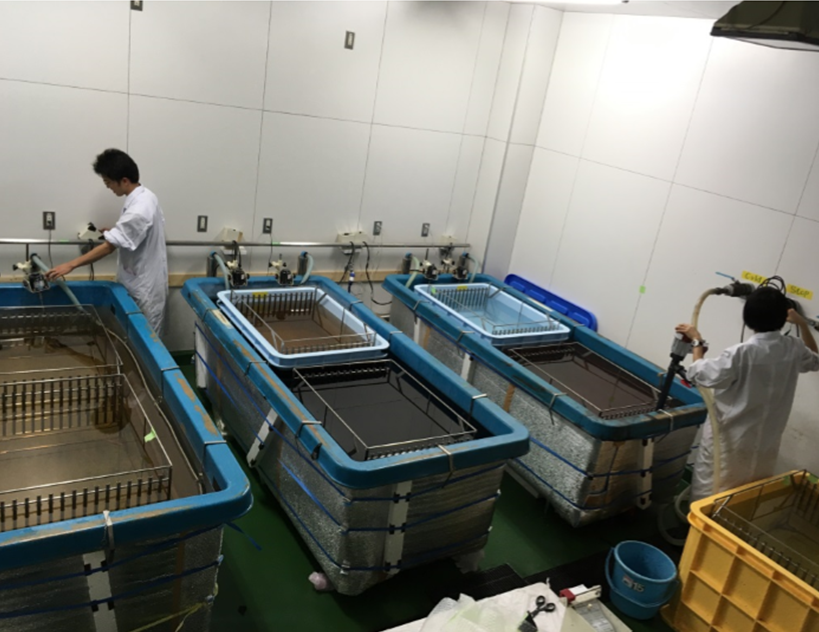
\includegraphics[width=100mm]{gennzou_condition.png}
  \caption{現像環境\label{fig:gennzou_bath}}
\end{figure}
\begin{figure}[htbp]
  \centering
     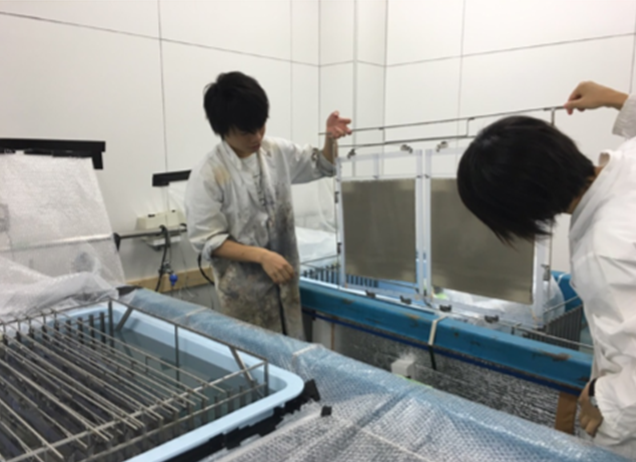
\includegraphics[width=100mm]{gennzou_turusi.png}
  \caption{現像の様子\label{fig:emulsion_turusi}}
\end{figure}
\begin{table}[htbp]
\centering
\caption{E07実験における現像タイムテーブル\label{tab:gennzou_timetable}}
\begin{center}
    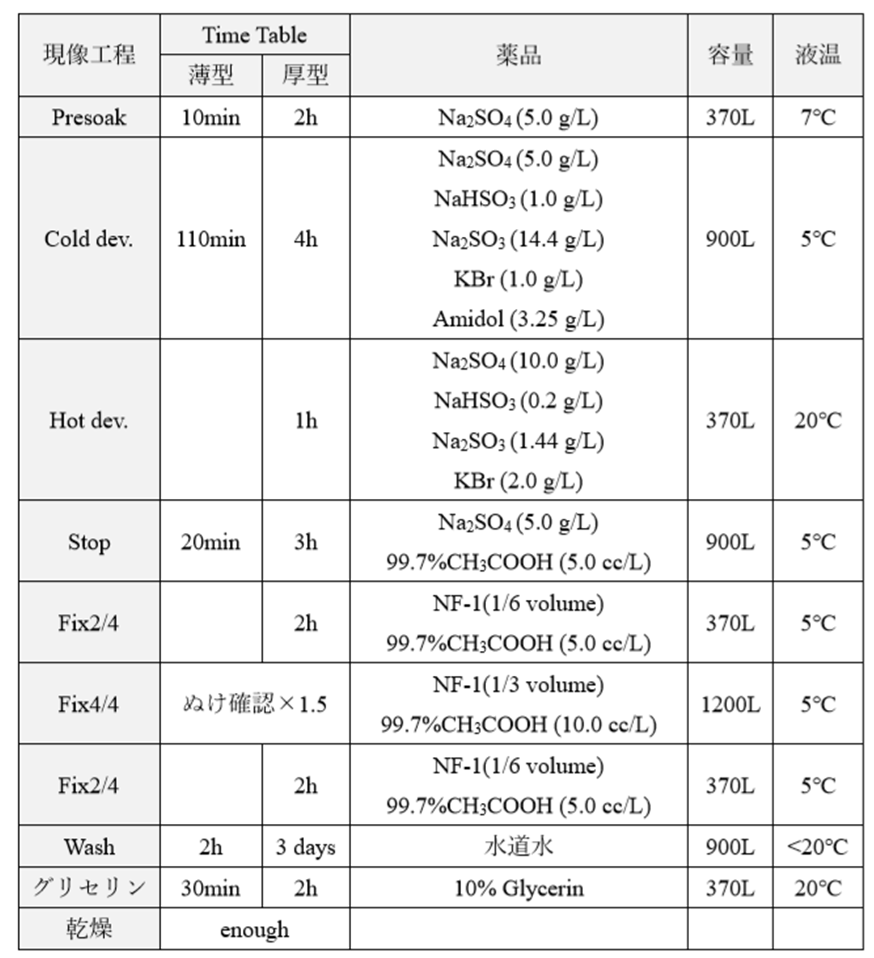
\includegraphics[width=150mm]{gennzou_timetable.png}
\end{center}
\end{table}


\newpage
\section{荷電粒子飛跡追跡の自動化}
\subsection{目的}
E373実験では人が約2.0×10$^4$本の$\Xi$$^-$候補を顕微鏡を使い静止点まで追跡した。
この追跡には約数年が必要となった。
先に記述したが、今年度実施されたJ-PARC E07実験ではハイブリッド-エマルジョン法によりE373実験の約10倍の統計量を検出することを目標にしている。
今回実施されたE07実験では、E373実験より精度の高い検出機であるSSDを使うことで追跡するべき候補飛跡を増やさないようにしている。
カウンターの情報と原子核乾板に記録された飛跡を一対一対応を付ける。
しかし、その条件であっても追跡すべき$\Xi$$^-$候補飛跡がE373実験の本数を超えることが予想されるため、
機械が自動で飛跡を静止点まで追跡するプログラムが必要になった。
\par
この章では$\Xi$$^-$候補飛跡のために使用・開発した要素技術を記述する。
\subsection{$\Xi$$^-$候補&beam認識に用いる画像処理}\label{image_process}
原子核乾板中に記録されている$\Xi$$^-$やK$^-$beamといった荷電粒子飛跡をコンピュータに認識されるために画像処理技術を使用する。
原子核乾板内部を撮影した画像に対して、
コントラスト処理、ガウシアンフィルタ処理、差分画像の二値化処理の順に実施する。
この画像処理工程により、画像中に記録されている荷電粒子飛跡の像を輝度値情報として取得する。
\par
ここでは画像処理工程に使用する、コントラスト処理、ガウシアンフィルタ処理、差分画像の二値化処理
について処理内容について詳細に記載する。
\subsubsection{コントラスト処理}
原子核乾板中を撮影した画像は、画像を撮影した原子核乾板の位置により見え方が異なる。
図\ref{fig:diff_contrust}は同一乾板内で撮影した写真で、視野中心に見えるのは追跡対象にしている$\Xi$$^-$候補飛跡である。
二つの写真の違いは原子核乾板の位置で、左が上側乳剤層、右が下側乳剤層で撮影したものである。
図より撮影地点が異なれば画像のコントラストが大きく異なることが分かる。
そこで原子核乾板中で撮影した画像を、撮影地点によらず飛跡情報を取得するために画像のコントラストの違いをなくす必要がある。
\begin{figure}[htbp]
  \centering
      \begin{tabular}{c}
        % 1枚目の画像
        \begin{minipage}{0.5\hsize}
          \centering
            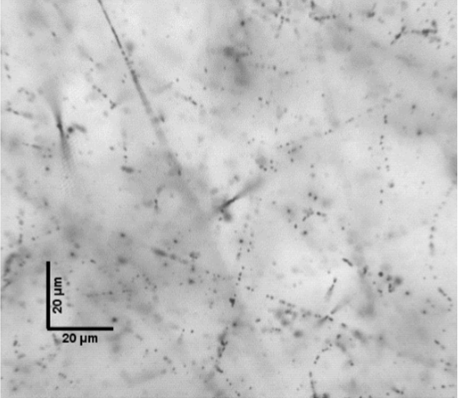
\includegraphics[clip, width=60mm]{emulsion_up.png}
            \hspace{1.6cm} (a)上側乳剤層中の$\Xi$$^-$候補飛跡
        \end{minipage}

        % 2枚目の画像
        \begin{minipage}{0.5\hsize}
          \centering
            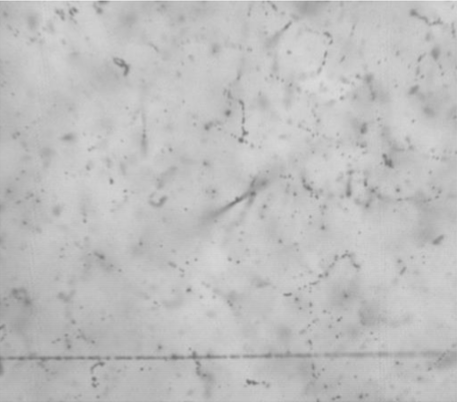
\includegraphics[clip, width=60mm]{emulsion_low.png}
            \hspace{1.6cm} (b)下側乳剤層中の$\Xi$$^-$候補飛跡
        \end{minipage}
    
      \end{tabular}
      \caption{撮影地点によるコントラストの違い\label{fig:diff_contrust}}
\end{figure}
\par
コントラストとは、画像の濃淡情報の分布の広さに関する性質で、画像の最大輝度を$I_{max}$、最小輝度を$I_{min}$とするとき式(\ref{eq:cont})で表す。
コントラスト処理に使う変化式はまた調べて記入する。
\begin{equation}
  C = \frac{I_{max} - I_{min}}{I_{max} + I_{min}}
\label{eq:cont}
\end{equation}
\par
画像のコントラストをよくするために用いる式は以下の通りである。
xは画像のある画素が持つ輝度値である。
\begin{equation}
  f(x) = 
  \begin{cases}
      0, & \text{$x = I_{min}$} \\
      255*\frac{x - I_{min}}{I_{max} - I_{min}}, & \text{$I_{min} < x < I_{max}$} \\
      255, & \text{$x = I_{max}$}
  \end{cases}
  \label{eq:cont_do}
\end{equation}
図\ref{fig:do_contrust_beforeandafter}は式(\ref{eq:cont_do})を使用して画像にコントラスト処理を施した画像である。
図の(c)、(d)を比較すると、コントラスト処理により画像の輝度値の明暗の幅が広がったことが分かる。
\begin{figure}[htbp]
  \centering
      \begin{tabular}{c}
        % 1枚目の画像
        \begin{minipage}{0.5\hsize}
          \centering
            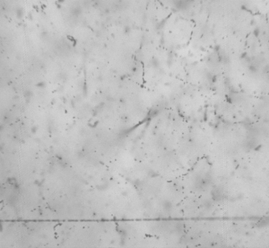
\includegraphics[clip, width=60mm]{row.png}
            \hspace{1.6cm} (a)コントラスト処理前
        \end{minipage}
        
        % 2枚目の画像
        \begin{minipage}{0.5\hsize}
          \centering
            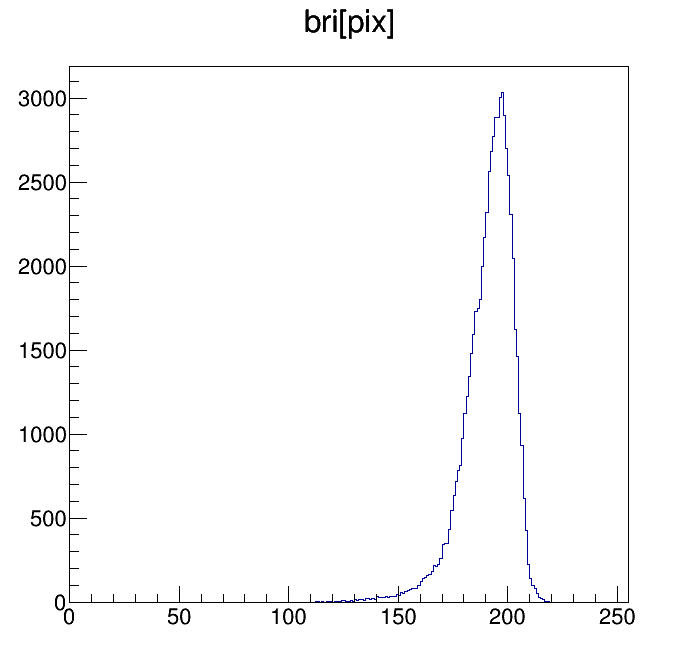
\includegraphics[clip, width=60mm]{row_hist.png}
            \hspace{1.6cm} (b)コントラスト処理前の一視野の輝度値分布
        \end{minipage}
        \\
        \\
        % 3枚目の画像
        \begin{minipage}{0.5\hsize}
          \centering
              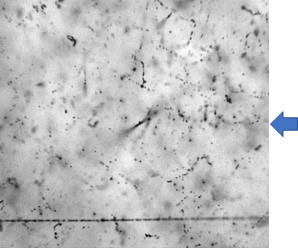
\includegraphics[clip, width=60mm]{cont.png}
              \hspace{1.6cm} (c)コントラスト処理後
          \end{minipage}
          
        % 4枚目の画像
        \begin{minipage}{0.5\hsize}
          \centering
              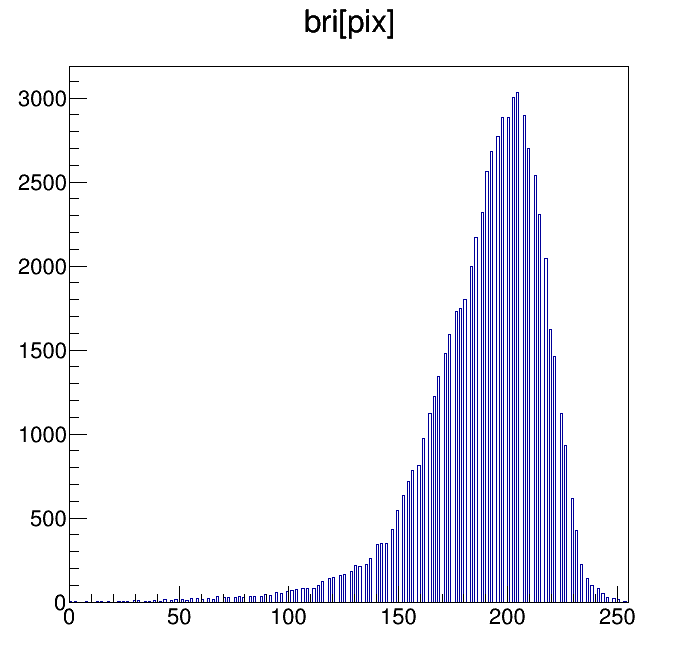
\includegraphics[clip, width=60mm]{cont_hist.png}
              \hspace{1.6cm} (d)コントラスト処理後の一視野の輝度値分布
        \end{minipage}
    
      \end{tabular}
      \caption{コントラスト処理によるコントラストの違い\label{fig:do_contrust_beforeandafter}}
\end{figure}
\newpage
\subsubsection{ガウシアンフィルタ処理}
撮影された画像には意図していないノイズが含まれている。
機械に飛跡を認識させるために、画像を構成する1つ1つのpixelに割り当てられた輝度値情報を利用する。
画像処理によりなめらかな濃淡変化を画像に与え、画像に含まれるノイズなどの不要な濃淡変動を軽減する。(平滑化)
\par
ガウシアンフィルタとは、画像の平滑化を行うために設定する平滑化フィルタの一例である。
フィルタによって覆われる領域内の画素の値がフィルタの原点に近いほど大きな重みをつけるが、この重みをガウス分布に近づけたフィルタを指す。
その際の二次元ガウス分布は式(\ref{eq:gausu})で表される。
\begin{equation}
  h_g(x,y) = \frac{1}{2\pi\sigma^2}exp(-\frac{x^2 + y^2}{2\sigma^2})
\label{eq:gausu}
\end{equation}
画像中のある画素を中心に指定範囲(カーネルサイズ)内で注目画素に近いほど輝度値の平均値を計算するときの重みを大きくするように処理をかけることである。
この式を使い、処理を実施した。
\par
図\ref{fig:do_gau_beforeandafter}は図\ref{fig:do_contrust_beforeandafter}で示した、
コントラスト処理後の画像に対してガウシアンフィルタ処理を実施した画像と画像の中央行の輝度値の変化をヒストグラムで示したものである。
処理前後の画像を比較すると、ガウシアンフィルタ処理を実施したことで画像全体の濃淡変化がなめらかになったことで、
画像ががぼけていることが分かる。
輝度値のヒストグラムを比較すると、処理前後により輝度値変化がなだらかになっていることが分かる。
図\ref{fig:do_gau_beforeandafter}のガウシアンフィルタ処理はカーネルサイズ = 51 で実施した。
\begin{figure}[htbp]
  \centering
      \begin{tabular}{c}
        % 1枚目の画像
        \begin{minipage}{0.5\hsize}
          \centering
            \includegraphics[clip, width=60mm]{cont.png}
            \hspace{1.6cm} (a)ガウシアンフィルタ処理前
        \end{minipage}
        
        % 2枚目の画像
        \begin{minipage}{0.5\hsize}
          \centering
            \includegraphics[clip, width=60mm]{cont_hist2.png}
            \hspace{1.6cm} (b)ガウシアンフィルタ処理前の画像における中央行の輝度値
        \end{minipage}
        \\
        \\
        % 3枚目の画像
        \begin{minipage}{0.5\hsize}
          \centering
              \includegraphics[clip, width=60mm]{gau2.png}
              \hspace{1.6cm} (c)ガウシアンフィルタ処理後
          \end{minipage}
          
        % 4枚目の画像
        \begin{minipage}{0.5\hsize}
          \centering
              \includegraphics[clip, width=60mm]{gau2_hist.png}
              \hspace{1.6cm} (d)ガウシアンフィルタ処理後の画像における中央行の輝度値
        \end{minipage}
    
      \end{tabular}
      \caption{ガウシアンフィルタ処理による輝度値の違い\label{fig:do_gau_beforeandafter}}
\end{figure}
\newpage
\subsubsection{差分の二値化}
二値化処理を実施するため、画像の白黒を反転させる。
ガウシアンフィルタ処理を施した画像から、コントラスト処理を施した画像の輝度値の差を取ることで白黒を反転する。
図\ref{fig:do_gau_beforeandafter}のガウシアンフィルタ処理後画像の輝度値から、
ガウシアンフィルタ処理前の輝度値情報を引いて作成したのが図\ref{fig:do_sub}である。
図\ref{fig:do_sub}を見れば分かるように差分を取ることで、黒色であった部分が白色に反転した。
これは、ヒストグラムに示した輝度値情報がガウシアンフィルタ処理前後により生じる違いによって生じる。
ガウシアンフィルタ処理後画像の輝度値が、ガウシアンフィルタ処理前画像の輝度値より大きい場合白色に、
小さい場合は黒になる。
\begin{figure}[htbp]
  \centering
      \begin{tabular}{c}
        % 1枚目の画像
        \begin{minipage}{0.5\hsize}
          \centering
            \includegraphics[clip, width=60mm]{sub.png}
            \hspace{1.6cm} (a)ガウシアンフィルタ処理後-処理前
        \end{minipage}

        % 2枚目の画像
        \begin{minipage}{0.5\hsize}
          \centering
            \includegraphics[clip, width=60mm]{sub_hist.png}
            \hspace{1.6cm} (b)差分処理後の画像における中央行の輝度値
        \end{minipage}
    
      \end{tabular}
      \caption{輝度値差分処理後の画像\label{fig:do_sub}}
\end{figure}
図\ref{fig:do_sub}を見ると、視野中心にある飛跡情報以外に多くの輝度値情報が記録されていることが分かる。
これらの情報は飛跡追跡を実施するのに不必要であり、飛跡の誤検出を招く恐れがある。
そこで、二値化処理により指定した輝度値以下のピクセルの輝度値をゼロにする。
これにより飛跡以外の不要な輝度値情報を消す。
\par
図\ref{fig:do_thre}は二値化処理前後の画像とその指定した行の輝度値を示したものである。
閾値を70に設定して二値化処理を実施した。
図より二値化処理により飛跡以外の不要な輝度値情報を消し去り、追跡に必要な輝度値情報を持つ画素のみ輝度値情報を保持していることが分かる。
\begin{figure}[htbp]
  \centering
      \begin{tabular}{c}
        % 1枚目の画像
        \begin{minipage}{0.5\hsize}
          \centering
            \includegraphics[clip, width=60mm]{thre.png}
            \hspace{1.6cm} (a)図\ref{fig:do_sub}(a)の二値化処理後画像
        \end{minipage}

        % 2枚目の画像
        \begin{minipage}{0.5\hsize}
          \centering
            \includegraphics[clip, width=60mm]{thre_hist.png}
            \hspace{1.6cm} (b)二値化処理後の画像における中央行の輝度値
        \end{minipage}
    
      \end{tabular}
      \caption{二値化処理後の画像\label{fig:do_thre}}
\end{figure}
\newpage
\subsection{座標変換}
追跡するべき飛跡情報はDetector座標系(SSD座標系)、Grid座標系(現像前座標系)、Stage座標系(現像後座標系)の3座標系で表すことができる。
Detector座標系はSSDで検出した飛跡情報を記録した座標系である。
原子核乾板に照射されているすべての荷電粒子飛跡の位置情報はすべてDetector座標系で記録されている。
\par
Grid座標系はemulsionにbeam照射をして現像をする前の座標系である。
Gridマークが照射された際の座標系であるため、beam照射の際に原子核乾板に照射された荷電粒子飛跡の位置情報原子核乾板版である。
\par
Stage座標系は顕微鏡で原子核乾板を観察する際の座標系である。
Stage上に乗せる際の傾きだけでなく、現像後の原子核乾板の伸縮が影響する。
\par
上述した通り、SSDで検出された$\Xi$$^-$候補飛跡はDetector座標系で記録されている。
検出された候補飛跡を原子核乾板で観察するためにはDetector座標系、Grid座標系、Stage座標の座標間の変換を適切に行う必要がある。
その座標間の変換を適切に行うためにaffine変換を使用する。
\par
\begin{equation}
  \left(
    \begin{array}{c}
    x \\
    y
    \end{array}
  \right)
  =
  \left(
    \begin{array}{cc}
      a & b \\
      c & d
    \end{array}
  \right)
  \left(
    \begin{array}{c}
      X \\
      Y
    \end{array}
  \right)
  +
  \left(
    \begin{array}{c}
      p \\
      q
    \end{array}
  \right)
\label{eq:affine}
\end{equation}
式(\ref{eq:affine})を使い、座標変換を行う。
x,yが座標変換後の座標、X,Yが座標変換前の座標、2行2列の行列が線形変換、p,qが平行移動の成分になる。
x,yとX,Yが対応している地点を3点以上検出し、式を解くことで各変換パラメータを出取得できる。
その変換パラメータを使い、対応がついていない地点の座標を推定する。
\subsection{自動追跡の要素技術}
荷電粒子自動追跡を実施するために様々な技術開発が必要である。
SSDと原子核乾板乾、乾板間の位置差を取得するために使用するbeamパターンマッチ。
原子核乾板の乳剤層と非乳剤層を識別するための表面認識。
そして、原子核乾板中に記録された荷電粒子飛跡を自動で追跡するためのプログラム開発。
\par
ここでは、beamパターンマッチ、表面認識、自動追跡プログラムの詳細について記載する。
\subsubsection{beamパターンマッチ}
カウンターと原子核乾板の位置ズレや乾板間の位置ズレを正確に取得する手法としてbeamパターンマッチという手法が開発された\cite{daisuke}。
図\ref{fig:beam_mosikizu1}、\ref{fig:beam_mosikizu2}はパターンマッチの模式図である。
系1と系2に記録されたbeamの形状が変化しておらず、互いの系において座標が異なる場合、使用できる。
パターンマッチをするために系1と系2に記録されたbeamの座標の差分を総当たりで計算をする。
この二つのbeamパターンを適当に一つの座標系に並べ、すべての組み合わせでベクトルを引く。
系1のbeam一点に対して複数のbeamの位置差をとることになるので、計算後系1のbeam一点に対して複数のベクトルが引けることになる。
この作業をすべてのbeamで実施したのち、そのすべてのベクトルの原点を合わせて二次元平面で集計する。
このとき、系1と系2がある数値分ずれている場合、その数値分ずれたベクトルが多く集計され、その他のベクトルはほとんど集計されないことになる。
これにより、系1と系2の間に一定値のずれが存在している場合の位置ズレが取得できる。
\par
この手法により座標系間の位置対応、乾板間の位置対応をつけ、上述したaffine変換やtrack追跡に使用する。
\begin{figure}[htbp]
  \centering
     \includegraphics[width=90mm]{beam_pattern1.png}
  \caption{beamパターンマッチ模式図\label{fig:beam_mosikizu1}}
\end{figure}
\begin{figure}[htbp]
  \centering
     \includegraphics[width=140mm]{beam_pattern2.png}
  \caption{beamパターンマッチ模式図\label{fig:beam_mosikizu2}}
\end{figure}
\begin{figure}[htbp]
  \centering
     \includegraphics[width=120mm]{nodata.png}
\end{figure}
\newpage
\subsubsection{表面認識}
原子核乾板中の飛跡を認識するために、原子核乾板の乳剤と非乳剤の地点を正確に捉える必要がある。
図\ref{fig:do_hyoumenn_outin_image}(a)、(b)は原子核乾板の乳剤層と非乳剤層で撮影した画像である。
乳剤中で撮影した画像の場合は飛跡等が記録されているが、非乳剤層では記録されない。
この画像に対して画像処理を実施したのが図\ref{fig:do_hyoumenn_outin_image}(c)、(d)である。
図より乳剤層か非乳剤層かにより画像処理後の画像中で輝度値情報を持つピクセルの数が異なることが分かる。
輝度値情報を持つピクセルの数により乳剤層か否かを判断する。
\begin{figure}[htbp]
  \centering
      \begin{tabular}{c}
        % 1枚目の画像
        \begin{minipage}{0.5\hsize}
          \centering
            \includegraphics[clip, width=60mm]{emulsion_in.png}
            \hspace{1.6cm} (a)乳剤層
        \end{minipage}
        
        % 2枚目の画像
        \begin{minipage}{0.5\hsize}
          \centering
            \includegraphics[clip, width=60mm]{emulsion_out.png}
            \hspace{1.6cm} (b)非乳剤層
        \end{minipage}
        \\
        \\
        % 3枚目の画像
        \begin{minipage}{0.5\hsize}
          \centering
              \includegraphics[clip, width=60mm]{emul_in_thre.png}
              \hspace{1.6cm} (c)画像処理後(乳剤層)
          \end{minipage}
          
        % 4枚目の画像
        \begin{minipage}{0.5\hsize}
          \centering
              \includegraphics[clip, width=60mm]{emul_out_thre.png}
              \hspace{1.6cm} (d)画像処理後(非乳剤層)
        \end{minipage}
    
      \end{tabular}
      \caption{原子核乾板内外での違い\label{fig:do_hyoumenn_outin_image}}
\end{figure}
\newpage
\par
顕微鏡操作し、乾板中の焦点が合っている箇所のZ軸だけを動かし3 $\mu$m間隔で画像を撮影し、画像処理を実施する。
その操作を行い、輝度値情報を持つピクセルの数を縦軸、Z座標を横軸に取り作成したのが図\ref{fig:hyoumenn_kidoti}である。
図より輝度値が急激に変化している箇所が4箇所ほど存在している。
その部分が乳剤層と非乳剤層の境界になる。
各境界面を認識する閾値を設定し、乳剤層である座標を求める。
\begin{figure}[htbp]
  \centering
     \includegraphics[width=90mm]{hyoumenn.png}
  \caption{原子核乾板の撮影か所による白ピクセル数の推移\label{fig:hyoumenn_kidoti}}
\end{figure}
\newpage
\subsubsection{荷電粒子飛跡追跡}\label{track_following}
原子核乾板中に記録された荷電粒子飛跡を認識するために最も重要なのは、荷電粒子飛跡の重心を正確にとらえることである。
飛跡の重心をとらえるために、乾板中の荷電粒子飛跡の写真を撮影し、
\ref{image_process}に記した画像処理を用いて画像から重心を取得する。
\par
追跡する荷電粒子の位置情報から、飛跡が画像の視野中心にあるとする。
追跡する荷電粒子の角度情報をもとに飛跡に沿い、常に視野中心にあるように顕微鏡のx,y方向を駆動させながら、現像前z=-6×$\tan$$\theta$ $\mu$m間隔で10枚の画像を撮影する。
10枚の画像すべてに上述した画像処理を施し、輝度値情報が反転した画像に変換する。
追跡の際に、荷電粒子飛跡が常に画像中心にあるようにして撮影をしているので、画像中に記録された輝度情報をすべて使う必要はない。
また、追跡している$\Xi$$^-$候補飛跡と同様の角度で照射されている飛跡を誤追跡する可能性も生じる。
そのため飛跡の重心検出処理の前に、画像処理で画像の領域(mask)を設定し、領域外の輝度情報を消した画像にしている。
図\ref{fig:tuiseki_gazou}は原子核乾板中に記録された荷電粒子飛跡を撮影した画像に対して画像処理を行った結果である。
画像は、指定した範囲内に記録された荷電粒子飛跡を拡大している。
(a)が元画像、(b)がコントラスト処理後の画像、(c)がガウシアンフィルタ処理後の画像(カーネルサイズ = 51×51)、
(d)が(c)-(b)の差分画像、(e)が二値化処理後の画像(閾値 = 100)である。
\begin{figure}[htbp]
  \centering
     \includegraphics[width=60mm]{angle_in_eml.png}
  \caption{原子核乾板中の飛跡の角度定義}
\end{figure}
\begin{figure}[htbp]
  \centering
     \includegraphics[width=120mm]{tuiseki_gazou.png}
  \caption{撮影した画像に対する画像処理\label{fig:tuiseki_gazou}}
\end{figure}
\newpage
\par
mask内のみの情報を残した画像を使い、重心検出を行う。
画像処理後の画像をすべて積層させる。
画像中心に$\Xi$$^-$候補飛跡が写るようにして原子核乾板内の写真を撮影しているため、
複数の画像に$\Xi$$^-$候補飛跡は記憶されている。
そのため、積層画像は$\Xi$$^-$候補飛跡である部分の画素の持つ輝度値情報は大きな値となり、
画像一枚に単発で記録されてる飛跡やgrain情報の画素の持つ輝度値情報は小さな値となる。
積層画像に対して閾値を設け、その値によって二値化をする。
これにより、画像中には追跡している飛跡の輝度値情報のみ残る。
図\ref{fig:sekisou_nitika}は実際の積層画像に対して二値化処理を実施した結果を示したものである。
(f)は画像処理した10枚の画像の輝度値を積層した画像、(g)はその画像に対して二値化処理をした結果を示したものである。
図より閾値を調整することで、積層画像から追跡している飛跡情報のみを残すことができることが分かる。
二値化後の積層画像に残った輝度値のまとまりから重心を計算し、
原子核乾板中の飛跡座標にする。
\begin{figure}[htbp]
  \centering
     \includegraphics[width=110mm]{tuiseki_gazou2.png}
  \caption{積層画像に対する二値化処理\label{fig:sekisou_nitika}}
\end{figure}
\par
原子核乾板中に記録された荷電粒子飛跡が直線的に記録されているのならば、撮影した画像をそのまま積層することで、飛跡の重心を算出することができる。
しかし、追跡している飛跡の角度と予測した角度が異なるまま撮影した画像をそのまま積層すると、追跡している荷電粒子飛跡の重心を検出することができない。
そのため、飛跡追跡では撮影した画像の積層方法を変化させている。
図\ref{fig:sekisou_mosikizu}は積層方法の模式図である。
撮影した画像をただ積層するだけではなく、ずらして積層させる。
これにより、ただ積層させる場合より適切に飛跡の重心を算出する。
この手法によって複数飛跡候補が出現した場合は、追跡してきた飛跡の角度と予測位置のズレからより適切な飛跡を選択する。
この操作により飛跡を検出できなかった場合は画像の撮影間隔を現像前z=-4×$\tan$$\theta$ $\mu$mで撮影し、同様の処理を行うことで飛跡を検出する。
\begin{figure}[htbp]
  \centering
     \includegraphics[width=110mm]{sekisou_step3.png}
  \caption{画像の積層方法模式図\label{fig:sekisou_mosikizu}}
\end{figure}
\par
この画像撮影と飛跡の重心検出を繰り返すことで、原子核乾板内に記録された飛跡を乾板をまたいで追跡し、静止点まで追跡する。
静止点まで追跡し、追跡した飛跡が消失した場合は積層画像を撮影する。
すべての飛跡を追跡した後に積層画像を確認することで、イベントかどうかの判断をする。
\par
開発したプログラムを用いて、E373実験で検出されたNagara Eventを追跡した。
図\ref{fig:nagara_sekisou}はNagara Eventを生成した飛跡を追跡し、追跡した飛跡が消失した地点で撮影した積層画像である。
図より、静止点近傍まで追跡をし、積層画像を確認することでイベントかどうかの判断ができることが分かる。
\begin{figure}[htbp]
  \centering
     \includegraphics[width=60mm]{superimpsed_org4.png}
  \caption{Nagara Eventを追跡して作成された積層画像\label{fig:nagara_sekisou}}
\end{figure}
\newpage
\subsection{自動追跡の実施とその結果}
上述した要素技術を使用して、実際に原子核乾板に記録された荷電粒子飛跡を光学顕微鏡を使用して追跡する。
自動追跡のためにはSSDで検出された$\Xi$$^-$候補を原子核乾板で検出し、
検出した飛跡を下流の原子核乾板へと繋いで追跡をする。
その際に必要となるのは各座標系間の変換パラメータの算出である。
Grid座標系、Stage座標系の間の変換パラメータを算出するために、原子核乾板を顕微鏡に貼り付けた際のGridマーク測定が必要になる。
Detector座標系、Grid座標系間の変換パラメータを算出するために、P-barによるパターンマッチが必要になる。
\par
各座標系間の変換パラメータを算出後はSSDの情報を使い、原子核乾板薄型一枚目をスキャンし$\Xi$$^-$候補飛跡を検出する。
検出した$\Xi$$^-$候補飛跡の角度と位置差から下流の原子核乾板に追跡する候補を選択し、追跡する。
\par
下流の原子核乾板に接続し追跡する際に、原子核乾板に垂直に照射されているK$^-$beamによるパターンマッチが必要になる。
このパターンマッチにより原子核乾板間の位置ズレを算出する。
乾板間のズレを算出し、上流の原子核乾板で検出した$\Xi$$^-$候補飛跡を下流の原子核乾板で検出した後に自動追跡を行う。
\par
ここでは自動追跡実施の際に必要となる作業内容の詳細や実際に追跡した際の結果について記述する。
\newpage
\subsubsection{原子核乾板の顕微鏡貼り付け時の座標変換パラメータの算出}
原子核乾板で追跡やスキャンを実施する前に、
原子核乾板を顕微鏡ステージに張り付けた際の回転や現像前後の変化を原子核乾板に照射されたGridマークを測定することで取得する必要がある。
SSDで検出した$\Xi$$^-$候補を顕微鏡で観察するために、Detector座標系、Grid座標系、Stage座標系の間の変換パラメータを適切に算出する必要がある。
このGridマークの測定によりGrid座標系、Stage座標系の2座標系間の変換パラメータを算出する。
\begin{figure}[htbp]
  \centering
     \includegraphics[width=140mm]{grid2stage.png}
  \caption{測定したGridマークと対応するGridマークネガ\label{fig:grid2stage}}
\end{figure}
\par
図\ref{fig:grid2stage}は顕微鏡に張り付けた原子核乾板中測定したGridマークとそれに対応するGridマークネガの場所を示している。
赤丸で囲んだ地点を測定した。
図に示したように、原点となる中心のGridマークと原子核乾板の四隅付近の記録されているGridマークのStage座標を記録する。
そして、測定したGridマークに対応する地点のネガにおけるGridマークの座標を記録し、上述した座標変換を行うことで、
Grid座標系、Stage座標系の2座標系間の変換パラメータを算出する。
算出したGrid座標系、Stage座標系の2座標系間の変換パラメータは、原子核乾板を顕微鏡に貼るたびに測定する必要がある。
\newpage
\subsubsection{P-barパターンマッチ}
検出器の情報から選び出された$\Xi$$^-$候補を、
SSDの情報を使い薄型乾板1枚目(pl01)で$\Xi$$^-$候補飛跡として検出するために、
SSDと原子核乾板の座標系の位置合わせを行う必要がある。
原子核乾板にはSSDとemulsionの照射時の位置差を取得するために反陽子ビームが照射されている。
反陽子beamを使い、上述したbeamパターンマッチを実施する。
照射されているのは乾板の四つ角1cm1cmの領域であり、SSDと原子核乾板に対して垂直に照射されている。
照射されている反陽子beamの濃度は1平方センチあたり10$^4$である。
K$^-$beamは乾板に対して10$^6$照射されており、SSDとemulsionのパターンマッチをするには密に照射されているためp-barが必要になる。
\begin{figure}[htbp]
  \centering
     \includegraphics[width=140mm]{pbar_mosikizu.png}
  \caption{P-barパターンマッチ模式図\label{fig:pbar_mosikizu}}
\end{figure}
\par
角から1cmずつ内陸側に移動し、そこで5mm×5mmの領域をスキャンする。
上側乳剤層と下側乳剤層をスキャンし、baseを挟んで接続された垂直なbeamを選び出すことで、原子核乾板薄型一枚目での飛跡集団のパターンを取得する。
また、SSDに記録された垂直な飛跡集団を選び出すことでSSDに記録された飛跡集団のパターンを取得する。
図\ref{fig:pbar_pattern}はスキャンにより取得したbeamとSSDで検出したbeamをプロットしたものである。
左が原子核乾板に記録された垂直なbeam、右がSSDで検出した垂直なbeamである。
二つのグラフの大きさは、それぞれのスキャン範囲の大きさに対応している。
この二つの座標系のbeamの対応を上述したbeamパターンマッチによりつける。
SSDで検出したbeamのプロットの中で赤くプロットされている部分が、原子核乾板に記録されたbeamが対応している部分である。
このように薄型原子核乾板の四か所においてbeam位置の対応をつけることでDetector座標系(SSD座標系)、Grid座標系(現像前座標系)の対応をつける。
\begin{figure}[htbp]
  \centering
     \includegraphics[width=90mm]{pbar_pattern.png}
  \caption{P-barパターンマッチ\label{fig:pbar_pattern}}
\end{figure}
\newpage
\subsubsection{$\Xi$$^-$候補飛跡の選択}\label{pl01_track}
追跡するために、SSDで検出した$\Xi$$^-$候補とpl01に記録された荷電粒子飛跡の対応をつける。
先述したP-barパターンマッチにより、SSDと原子核乾板の座標の対応がついており、
Detector座標系からGrid座標系へのaffineパラメータを求められていることが前提である。
図\ref{fig:pl01_mosikizu}は原子核乾板に記録された飛跡からSSDで検出した$\Xi$$^-$候補を選び出す過程を模式図で示したものである。
affineパラメータにより、SSDで検出した$\Xi$$^-$候補が原子核乾板上でどの位置に記録されているかを求める。
そして、SSDで検出された$\Xi$$^-$候補の位置情報と角度情報を使い、$\Xi$$^-$候補の位置を薄型原子核乾板1枚目のbase上面まで外挿する。
これにより$\Xi$$^-$候補の薄型原子核乾板1枚目のbase上面における位置がおおよそ分かる。
この薄型原子核乾板1枚目のbase上面における位置情報と角度情報を合わせてprediction(pred)とする。
\par
predの座標を中心にして$\Xi$$^-$候補の角度により、原子核乾板中をスキャンする範囲を設定する。
図の赤枠がscan範囲とする。
設定した範囲を元に、原子核乾板の上側乳剤層、下側乳剤層をscanし、原子核乾板中に記録されている荷電粒子飛跡を検出する。
検出した飛跡の中から、baseをまたいで繋がるものを薄型一枚目を通過している飛跡(basetrack)として記録する。
basetrackは位置情報、角度情報を持っている。
predとbasetrackの中から、位置差、角度差が小さな飛跡を追跡対象として下流の原子核乾板に接続し、飛跡追跡を行う。
\begin{figure}[htbp]
  \centering
     \includegraphics[width=140mm]{pl01_mosikizu.png}
  \caption{$\Xi$$^-$候補飛跡模式図\label{fig:pl01_mosikizu}}
\end{figure}
\newpage
\par
$\Xi$$^-$候補は、KURAMAスペクトロメータのデータを解析により多数の荷電粒子情報の中から選出する。
$\Xi$$^-$粒子検出の手順は以下の通りである。
\begin{enumerate}
  \item スペクトロメータの解析で(K$^-$,K$^+$)イベントを選び出す。
  \item SSDのhitの中からdEが大きいものを選び出し、4層全てで検出した場合にtrackを作成する。
  \item vertex・角度の情報を使い、$\Xi$$^-$粒子を識別する。
\end{enumerate}
\par
$\Xi$$^-$stopの可能性の高いものから解析できるように異なるcut条件で追跡する$\Xi$$^-$候補を選出した。
表\ref{tab:guzai_list}はそれをまとめたものである。
作成された$\Xi$$^-$リストの中からstop確立の高いcut条件cut1のものから追跡を行い、その後cut2、cut3と実施していく。
\begin{table}[htbp]
  \centering
  \caption{118スタックの解析結果\label{tab:guzai_list}}
  \begin{center}
      \includegraphics[width=150mm]{guzai_list.png}
  \end{center}
\end{table}
\newpage
\par
SSDで検出した$\Xi$$^-$候補の位置情報、角度情報を使い、Mod009薄型乾板一枚目をスキャンした。
スキャンに使用した$\Xi$$^-$候補のリストは表\ref{tab:guzai_list}のcut1により作成されたものである。
スキャンした結果から、$\Xi$$^-$候補飛跡の位置と角度が似ているものを$\Xi$$^-$候補飛跡の追跡候補として選び出した。
図\ref{fig:ssd_pl01}はSSDで検出した$\Xi$$^-$候補とスキャン結果から検出した$\Xi$$^-$候補飛跡の位置差を示している。
SSDよって検出した$\Xi$$^-$候補と検出した飛跡の位置座標が同じであれば図の原点にプロットされる。
そのため適切に予測、検出がされていれば、SSDで検出された$\Xi$$^-$候補をもとに薄型乾板一枚目で検出された飛跡は
図の中心付近にプロットされる。
それに対して、原子核乾板に記録されているバックグラウンドを飛跡として検出している場合、
図の中心から外れた場所に位置差のデータ点がプロットされる。
このデータ点すべてを追跡候補として下流の原子核乾板に接続し、静止点まで追跡する。
図\ref{fig:ssd_pl01}は536本の$\Xi$$^-$候補をもとに薄型乾板一枚目スキャンし検出した$\Xi$$^-$候補飛跡との位置差をプロットした結果である。
データ点は536個存在している。
\begin{figure}[htbp]
  \centering
     \includegraphics[width=80mm]{dx_dy.png}
  \caption{原子核乾板のスキャンから検出した荷電粒子飛跡とSSDで検出した$\Xi$$^-$候補の位置差\label{fig:ssd_pl01}}
\end{figure}
\begin{figure}[htbp]
  \centering
      \begin{tabular}{c}
        % 1枚目の画像
        \begin{minipage}{0.5\hsize}
          \centering
            \includegraphics[clip, width=70mm]{dx_ax.png}
            \hspace{1.6cm} 
            \caption{原子核乾板のスキャンから検出した荷電粒子飛跡とSSDで検出した$\Xi$$^-$候補のx方向の位置差、角度差\label{fig:ssd_pl01_x}}
        \end{minipage}
        
        % 2枚目の画像
        \begin{minipage}{0.5\hsize}
          \centering
            \includegraphics[clip, width=70mm]{dy_ay.png}
            \hspace{1.6cm} 
            \caption{原子核乾板のスキャンから検出した荷電粒子飛跡とSSDで検出した$\Xi$$^-$候補のy方向の位置差、角度差\label{fig:ssd_pl01_y}}
        \end{minipage}
      \end{tabular}
\end{figure}
\par
図\ref{fig:ssd_pl01}を見ると、
SSDで検出した$\Xi$$^-$候補と原子核乾板のスキャンから検出した荷電粒子飛跡の位置差のデータ点が図の原点付近にないことが分かる。
原子核乾板のスキャンを開始する前には原子核乾板に照射されたGridマークの座標を取得することで、座標変換のパラメータを取得しスキャンを実施している。
そのため、Gridマーク座標記録の数を増加し、原子核乾板全域において適切に変換可能なパラメータの算出をすることで、
原点付近にデータ点が近づくのかを検証した。
\newpage
\par
図\ref{fig:grid5}はMod013pl01に記録されたGridと、Gridマークの検出点と予想点の位置差を示したものである。
赤丸で囲われた5点のGridマーク測定により算出したaffineパラメータを使用し、pl01のGridマーク測定を実施した。
検出点と予想点の差を示した矢印が大きくなるほどズレが大きいことを示している。
位置差を示した図の下部に青い矢印で示した部分がある。
ここを確認すると、原子核乾板の下辺部分にて100 $\mu$m程度の差が生じている。
そこで、affineパラメータを算出するために測定するGridマークの数を9点に増やした結果が図\ref{fig:grid9}である。
図\ref{fig:grid9}の位置差を確認すると、5点測定の際に生じていた位置差が50 $\mu$mほどになった。
これにより、SSDとpl01のdx、dy分布が50 $\mu$m程度に収まると考え、pl01の測定を実施した。
\par
図\ref{fig:dxdy5}はGridマークを5点測定して算出したaffineパラメータを使いpl01のスキャンを実施した結果、
図\ref{fig:dxdy9}はGridマークを9点測定して算出したaffineパラメータを使いpl01のスキャンを実施した結果である。
これらの図を比較すると、Gridマークの測定点を増加させても、SSDとpl01の位置差が収束しないことが分かる。
しかし、SSDからpl01への外挿距離を変化させて位置差と角度の相関を示したのが図\ref{fig:ssd_pl01_x02}~\ref{fig:ssd_pl01_y_02}である。
外挿距離の変化に伴って、位置差に変化が生じるため$\Xi$$^-$候補飛跡を検出できていると判断し、データ点すべてを追跡した。
\begin{figure}[htbp]
  \centering
     \includegraphics[width=150mm]{grid5_pl01scan.png}
  \caption{薄型乾板に記録されたGridマークと、5点のGridマーク測定により算出したパラメータを使用した際のGridマークの検出点と予想点の位置差\label{fig:grid5}}
\end{figure}
\begin{figure}[htbp]
  \centering
     \includegraphics[width=150mm]{grid9_pl01scan.png}
  \caption{薄型乾板に記録されたGridマークと、9点のGridマーク測定により算出したパラメータを使用した際のGridマークの検出点と予想点の位置差\label{fig:grid9}}
\end{figure}
\begin{figure}[htbp]
  \centering
      \begin{tabular}{c}
        % 1枚目の画像
        \begin{minipage}{0.5\hsize}
          \centering
            \includegraphics[clip, width=70mm]{dx_dy_grid5.png}
            \hspace{1.6cm} 
            \caption{Gridマーク5点測定による原子核乾板のスキャンから検出した荷電粒子飛跡とSSDで検出した$\Xi$$^-$候補の位置差\label{fig:dxdy5}}
        \end{minipage}
        
        % 2枚目の画像
        \begin{minipage}{0.5\hsize}
          \centering
            \includegraphics[clip, width=70mm]{dx_dy_grid9.png}
            \hspace{1.6cm} 
            \caption{Gridマーク9点測定による原子核乾板のスキャンから検出した荷電粒子飛跡とSSDで検出した$\Xi$$^-$候補の位置差\label{fig:dxdy9}}
        \end{minipage}
      \end{tabular}
\end{figure}
\begin{figure}[htbp]
  \centering
      \begin{tabular}{c}
        % 1枚目の画像
        \begin{minipage}{0.5\hsize}
          \centering
            \includegraphics[clip, width=70mm]{ssdpl01_x_02.png}
            \hspace{1.6cm} 
            \caption{$\Xi$$^-$候補のx方向の位置差、角度差 外装距離-0.2 mm\label{fig:ssd_pl01_x_02}}
        \end{minipage}
        
        % 2枚目の画像
        \begin{minipage}{0.5\hsize}
          \centering
            \includegraphics[clip, width=70mm]{ssdpl01_y_02.png}
            \hspace{1.6cm} 
            \caption{$\Xi$$^-$候補のy方向の位置差、角度差 外装距離-0.2 mm\label{fig:ssd_pl01_y_02}}
        \end{minipage}
      \end{tabular}
\end{figure}
\begin{figure}[htbp]
  \centering
      \begin{tabular}{c}
        % 1枚目の画像
        \begin{minipage}{0.5\hsize}
          \centering
            \includegraphics[clip, width=70mm]{ssdpl01_x02.png}
            \hspace{1.6cm} 
            \caption{$\Xi$$^-$候補のx方向の位置差、角度差 外装距離0.2 mm\label{fig:ssd_pl01_x02}}
        \end{minipage}
        
        % 2枚目の画像
        \begin{minipage}{0.5\hsize}
          \centering
            \includegraphics[clip, width=70mm]{ssdpl01_y02.png}
            \hspace{1.6cm} 
            \caption{$\Xi$$^-$候補のy方向の位置差、角度差 外装距離0.2 mm\label{fig:ssd_pl01_y02}}
        \end{minipage}
      \end{tabular}
\end{figure}
\newpage
\subsubsection{K$^-$beamパターンマッチ}
beam照射は、エマルジョンカセットに13枚の原子核乾板を入れ、真空度を保ちbeam照射中に原子核乾板がずれないようにして実施した。
しかし、人の手でカセットに入れており、原子核乾板一枚一枚違いがあり、現像の前後での変形も一様ではないため、
各原子核乾板の位置情報は、原点を照射したGridマークの中心にしたときに対応しない。
そこで、beam照射時に原子核乾板に対して垂直に照射されているK$^-$beamを使い、上流乾板と下流乾板の位置の対応をつける。
これにより、上流の原子核乾板に記録されている$\Xi$$^-$候補飛跡と下流の原子核乾板に記録されている$\Xi$$^-$候補飛跡が一対一対応する。
\par
追跡を行うために上流の原子核乾板、下流の原子核乾板間に生じているズレを算出する。
図\ref{fig:beam_mosikizu}はパターンマッチの模式図である。
原子核乾板の各辺の中点付近をスキャンし、垂直に照射されているK$^-$beamを検出する。
図の赤い範囲がスキャンした範囲である。
上流の原子核乾板は下側乳剤層を約0.5 mm×0.5 mmの範囲をスキャンする。
下流の原子核乾板は上側乳剤層を約1 mm×1 mmの範囲をスキャンする。
スキャンした範囲に記録されたK$^-$beamをDetector座標系に直し、パターンマッチを行う。
\par
図\ref{fig:kbeam1}、\ref{fig:kbeam2}は実際のパターンマッチの結果である。
パターンマッチの結果求められた、四か所分の乾板間のズレを用いてDetector座標系、Grid座標系間の座標変換パラメータを算出する。
このパラメータは乾板を顕微鏡に貼るたびに変化するStage座標系とは関係ないため、
一度算出すれば何度も使用することができる。
\begin{figure}[htbp]
  \centering
     \includegraphics[width=70mm]{kbeam_pattern.png}
  \caption{K$^-$beamパターンマッチ模式図\label{fig:beam_mosikizu}}
\end{figure}
\begin{figure}[htbp]
  \centering
      \begin{tabular}{c}
        % 1枚目の画像
        \begin{minipage}{0.5\hsize}
          \centering
            \includegraphics[clip, width=70mm]{kbeam1.png}
            \hspace{1.6cm} 
            \caption{K$^-$beamパターンマッチ結果\label{fig:kbeam1}}
        \end{minipage}
        
        % 2枚目の画像
        \begin{minipage}{0.5\hsize}
          \centering
            \includegraphics[clip, width=70mm]{kbeam2.png}
            \hspace{1.6cm} 
            \caption{K$^-$beamパターンマッチ結果拡大図\label{fig:kbeam2}}
        \end{minipage}
      \end{tabular}
\end{figure}
\par
乾板間パターンマッチによるDetector座標系、Grid座標系間の座標変換パラメータ算出後、
$\Xi$$^-$候補飛跡を追跡するため座標変換パラメータを使い、
原子核乾板上の$\Xi$$^-$候補飛跡が記録されている地点に移動をする。
この移動により、追跡対象となる$\Xi$$^-$候補飛跡は顕微鏡の一視野内におさまるが、
視野中心に追跡対象の飛跡がない場合がある。
そのため、追跡対象の飛跡を視野中心に移動させるために、
追跡対象の飛跡付近でのK$^-$beamパターンマッチを実施する。
\par
図\ref{fig:kbeam_mosikizu2}は追跡時に追跡対象を視野中心に移動させるためのK$^-$beamパターンマッチの模式図である。
上流の原子核乾板の下側乳剤層下面における追跡対象付近のK$^-$beamと、
下流の原子核乾板の上側乳剤層上面における追跡対象付近のK$^-$beamのパターンマッチを行う。
これにより、追跡対象付近の位置ズレを正確に取得することができ、
追跡対象となる$\Xi$$^-$候補飛跡を視野中心に移動させて追跡を行うことができる。
\begin{figure}[htbp]
  \centering
     \includegraphics[width=100mm]{beam_mosikizu.png}
  \caption{$\Xi$$^-$候補飛跡追跡のためのK$^-$beamパターンマッチ模式図\label{fig:kbeam_mosikizu2}}
\end{figure}
\newpage
\subsubsection{$\Xi$$^-$候補飛跡追跡}
図\ref{fig:ssd_pl01}にプロットされたデータ点の数だけ追跡を行い、静止点まで追跡を行った。
図\ref{fig:tan_razial}、\ref{fig:tan_latelal}は飛跡追跡の飛跡の予測位置と検出位置の差を角度ごとに示したものである。
これを見ると、どの角度領域においても、予測と飛跡の検出地点の差が一定であることが分かる。
位置差が一定であることから、追跡する$\Xi$$^-$候補飛跡の角度に依存せず適切に追跡ができていることが分かる。
\begin{figure}[htbp]
  \centering
     \includegraphics[width=120mm]{radial.png}
  \caption{追跡時の予測地点と検出地点の位置差radial方向\label{fig:tan_razial}}
\end{figure}
\begin{figure}[htbp]
  \centering
     \includegraphics[width=120mm]{lateral.png}
  \caption{追跡時の予測地点と検出地点の位置差lateral方向\label{fig:tan_latelal}}
\end{figure}
\par
mod009で検出した$\Xi$$^-$候補飛跡535本すべてを追跡した結果、decayが16個、sigma stopが16個であった。
mod009の追跡ではHyper核eventは検出できなかったが、$\Xi$$^-$由来のeventを検出できているため、
今後追跡を継続して行うことでHyper核eventを検出できると考えられる。
\begin{figure}[htbp]
  \centering
      \begin{tabular}{c}
        % 1枚目の画像
        \begin{minipage}{0.5\hsize}
          \centering
            \includegraphics[clip, width=70mm]{sigma.png}
            \hspace{1.6cm} 
            \caption{検出したsigma stop\label{fig:sigma}}
        \end{minipage}
        
        % 2枚目の画像
        \begin{minipage}{0.5\hsize}
          \centering
            \includegraphics[clip, width=70mm]{decay.png}
            \hspace{1.6cm} 
            \caption{検出したdecay\label{fig:decay}}
        \end{minipage}
      \end{tabular}
\end{figure}
\par
今回追跡した約500本の候補を、pl01で検出し、pl12まで追跡する全工程での顕微鏡稼働時間は約50時間であった。
原子核乾板の問題や処理でのミスを考慮していない顕微鏡の稼働時間である。
$\Xi$$^-$リスト作成時のcut条件cut1では118modで約52300個の$\Xi$$^-$候補がある。
今回の追跡結果からcut1の追跡をすべて終了するのに必要な顕微鏡稼働時間は約218日間になる。
これは使用する光学顕微鏡が一台しかない場合のため、
複数台の光学顕微鏡を並列して稼働させることでより早くHyper核検出を可能とする。
\newpage
\section{まとめ}
私たちはE373実験の10倍の統計量を目指すE07実験Beam照射を実施した。
今後はsクォークを含む$\Lambda$、$\Xi$$^-$から粒子間の相互作用を求めれらる物理データを多く検出することが期待される。
\par
E07実験1st Runを2016年6月18日〜30日に、2nd Runを2017年5月~7月に実施した。
J-PARCでの放射能漏れによるbeam照射延期により、
原子核乾板に記録されたバックグラウンド消去のための強制現像退行処理を実施した。
これにより、荷電粒子飛跡を解析するために必要な原子核乾板の状態を作り出した。
\par
E07実験1st Runにて確立されたPacking手法を用いて、
2nd Runでは適切な真空度を保ったEmulsionCassetteをbeamline上に提供することができた。
また、1st Runで課題となったSUS箔の剥がれに対する対応策として、
Cassette固定冶具を作成した。
Cassette固定冶具を使用し2nd Runを実施したことで、
100回のCassette提供に対して、SUS箔の剥がれを1度に抑えることができた。
これにより、E07実験2nd Runのbeam照射を無事終了することができた。
\par
E07実験1st Run、2nd Runは実施され、全118modの現像を無事達成した。
\par
ハイブリッドエマルジョン法により、現像されたE07実験の原子核乾板の中に記録された$\Xi$$^-$候補飛跡を追跡した。
今までは先に行われたE373実験での原子核乾板を使用しての追跡のテストが行われていたが、
初めてE07実験の原子核乾板を使い自動飛跡追跡を実施した。
今回私が追跡した原子核乾板からはハイパー核事象は検出できなかったが、
$\Xi$$^-$由来の事象を複数検出できたことから、
今後追跡を継続していくことでNagara Eventのように重要な物理データを示すことのできるハイパー核事象を検出できると考えられる。

\newpage
\section*{付録}
\addcontentsline{toc}{section}{付録}
2nd RunでのMod019〜Mod118の真空度の結果を以下に⽰す。 
青のプロットが一度引き、オレンジが二度引き、緑が三度引き、黄色が四度引きの際の真空度のプロットである。
\afterpage{\clearpage}
%%#!platex 修士論文.tex
\begin{figure}[htbp]
    \centering
       \includegraphics[width=120mm]{vol_019.png}
  \end{figure}
  \begin{figure}[htbp]
    \centering
       \includegraphics[width=120mm]{vol_020.png}
  \end{figure}
  \begin{figure}[htbp]
    \centering
       \includegraphics[width=120mm]{vol_021.png}
  \end{figure}
  \begin{figure}[htbp]
    \centering
       \includegraphics[width=120mm]{vol_022.png}
  \end{figure}
  \begin{figure}[htbp]
    \centering
       \includegraphics[width=120mm]{vol_023.png}
  \end{figure}
  \begin{figure}[htbp]
    \centering
       \includegraphics[width=120mm]{vol_024.png}
  \end{figure}
  \begin{figure}[htbp]
    \centering
       \includegraphics[width=120mm]{vol_025.png}
  \end{figure}
  \begin{figure}[htbp]
    \centering
       \includegraphics[width=120mm]{vol_026.png}
  \end{figure}
  \begin{figure}[htbp]
    \centering
       \includegraphics[width=120mm]{vol_027.png}
  \end{figure}
  \begin{figure}[htbp]
    \centering
       \includegraphics[width=120mm]{vol_028.png}
  \end{figure}
  \begin{figure}[htbp]
    \centering
       \includegraphics[width=120mm]{vol_029.png}
  \end{figure}
  \begin{figure}[htbp]
    \centering
       \includegraphics[width=120mm]{vol_030.png}
  \end{figure}
  \begin{figure}[htbp]
    \centering
       \includegraphics[width=120mm]{vol_031.png}
  \end{figure}
  \begin{figure}[htbp]
    \centering
       \includegraphics[width=120mm]{vol_032.png}
  \end{figure}
  \begin{figure}[htbp]
    \centering
       \includegraphics[width=120mm]{vol_033.png}
  \end{figure}
  \begin{figure}[htbp]
    \centering
       \includegraphics[width=120mm]{vol_034.png}
  \end{figure}
  \begin{figure}[htbp]
    \centering
       \includegraphics[width=120mm]{vol_035.png}
  \end{figure}
  \begin{figure}[htbp]
    \centering
       \includegraphics[width=120mm]{vol_036.png}
  \end{figure}
  \begin{figure}[htbp]
    \centering
       \includegraphics[width=120mm]{vol_037.png}
  \end{figure}
  \begin{figure}[htbp]
    \centering
       \includegraphics[width=120mm]{vol_038.png}
  \end{figure}
  \begin{figure}[htbp]
    \centering
       \includegraphics[width=120mm]{vol_039.png}
  \end{figure}
  \begin{figure}[htbp]
    \centering
       \includegraphics[width=120mm]{vol_040.png}
  \end{figure}
  \begin{figure}[htbp]
    \centering
       \includegraphics[width=120mm]{vol_041.png}
  \end{figure}
  \begin{figure}[htbp]
    \centering
       \includegraphics[width=120mm]{vol_042.png}
  \end{figure}
  \begin{figure}[htbp]
    \centering
       \includegraphics[width=120mm]{vol_043.png}
  \end{figure}
  \begin{figure}[htbp]
    \centering
       \includegraphics[width=120mm]{vol_044.png}
  \end{figure}
  \begin{figure}[htbp]
    \centering
       \includegraphics[width=120mm]{vol_045.png}
  \end{figure}
  \begin{figure}[htbp]
    \centering
       \includegraphics[width=120mm]{vol_046.png}
  \end{figure}
  \begin{figure}[htbp]
    \centering
       \includegraphics[width=120mm]{vol_047.png}
  \end{figure}
  \clearpage
  \begin{figure}[htbp]
    \centering
       \includegraphics[width=120mm]{vol_048.png}
  \end{figure}
  \begin{figure}[htbp]
    \centering
       \includegraphics[width=120mm]{vol_049.png}
  \end{figure}
  \begin{figure}[htbp]
    \centering
       \includegraphics[width=120mm]{vol_050.png}
  \end{figure}
  \begin{figure}[htbp]
    \centering
       \includegraphics[width=120mm]{vol_051.png}
  \end{figure}
  \begin{figure}[htbp]
    \centering
       \includegraphics[width=120mm]{vol_052.png}
  \end{figure}
  \begin{figure}[htbp]
    \centering
       \includegraphics[width=120mm]{vol_053.png}
  \end{figure}
  \begin{figure}[htbp]
    \centering
       \includegraphics[width=120mm]{vol_054.png}
  \end{figure}
  \begin{figure}[htbp]
    \centering
       \includegraphics[width=120mm]{vol_055.png}
  \end{figure}
  \begin{figure}[htbp]
    \centering
       \includegraphics[width=120mm]{vol_056.png}
  \end{figure}
  \begin{figure}[htbp]
    \centering
       \includegraphics[width=120mm]{vol_057.png}
  \end{figure}
  \begin{figure}[htbp]
    \centering
       \includegraphics[width=120mm]{vol_058.png}
  \end{figure}
  \begin{figure}[htbp]
    \centering
       \includegraphics[width=120mm]{vol_059.png}
  \end{figure}
  \begin{figure}[htbp]
    \centering
       \includegraphics[width=120mm]{vol_060.png}
  \end{figure}
  \begin{figure}[htbp]
    \centering
       \includegraphics[width=120mm]{vol_061.png}
  \end{figure}
  \begin{figure}[htbp]
    \centering
       \includegraphics[width=120mm]{vol_062.png}
  \end{figure}
  \begin{figure}[htbp]
    \centering
       \includegraphics[width=120mm]{vol_063.png}
  \end{figure}
  \begin{figure}[htbp]
    \centering
       \includegraphics[width=120mm]{vol_064.png}
  \end{figure}
  \begin{figure}[htbp]
    \centering
       \includegraphics[width=120mm]{vol_065.png}
  \end{figure}
  \begin{figure}[htbp]
    \centering
       \includegraphics[width=120mm]{vol_066.png}
  \end{figure}
  \begin{figure}[htbp]
    \centering
       \includegraphics[width=120mm]{vol_067.png}
  \end{figure}
  \begin{figure}[htbp]
    \centering
       \includegraphics[width=120mm]{vol_068.png}
  \end{figure}
  \begin{figure}[htbp]
    \centering
       \includegraphics[width=120mm]{vol_069.png}
  \end{figure}
  \begin{figure}[htbp]
    \centering
       \includegraphics[width=120mm]{vol_070.png}
  \end{figure}
  \begin{figure}[htbp]
    \centering
       \includegraphics[width=120mm]{vol_071.png}
  \end{figure}
  \begin{figure}[htbp]
    \centering
       \includegraphics[width=120mm]{vol_072.png}
  \end{figure}
  \begin{figure}[htbp]
    \centering
       \includegraphics[width=120mm]{vol_073.png}
  \end{figure}
  \begin{figure}[htbp]
    \centering
       \includegraphics[width=120mm]{vol_074.png}
  \end{figure}
  \begin{figure}[htbp]
    \centering
       \includegraphics[width=120mm]{vol_075.png}
  \end{figure}
  \begin{figure}[htbp]
    \centering
       \includegraphics[width=120mm]{vol_076.png}
  \end{figure}
  \begin{figure}[htbp]
    \centering
       \includegraphics[width=120mm]{vol_077.png}
  \end{figure}
  \begin{figure}[htbp]
    \centering
       \includegraphics[width=120mm]{vol_078.png}
  \end{figure}
  \clearpage
  \begin{figure}[htbp]
    \centering
       \includegraphics[width=120mm]{vol_079.png}
  \end{figure}
  \begin{figure}[htbp]
    \centering
       \includegraphics[width=120mm]{vol_080.png}
  \end{figure}
  \begin{figure}[htbp]
    \centering
       \includegraphics[width=120mm]{vol_081.png}
  \end{figure}
  \begin{figure}[htbp]
    \centering
       \includegraphics[width=120mm]{vol_082.png}
  \end{figure}
  \begin{figure}[htbp]
    \centering
       \includegraphics[width=120mm]{vol_083.png}
  \end{figure}
  \begin{figure}[htbp]
    \centering
       \includegraphics[width=120mm]{vol_084.png}
  \end{figure}
  \begin{figure}[htbp]
    \centering
       \includegraphics[width=120mm]{vol_085.png}
  \end{figure}
  \begin{figure}[htbp]
    \centering
       \includegraphics[width=120mm]{vol_086.png}
  \end{figure}
  \begin{figure}[htbp]
    \centering
       \includegraphics[width=120mm]{vol_087.png}
  \end{figure}
  \begin{figure}[htbp]
    \centering
       \includegraphics[width=120mm]{vol_088.png}
  \end{figure}
  \begin{figure}[htbp]
    \centering
       \includegraphics[width=120mm]{vol_089.png}
  \end{figure}
  \begin{figure}[htbp]
    \centering
       \includegraphics[width=120mm]{vol_090.png}
  \end{figure}
  \begin{figure}[htbp]
    \centering
       \includegraphics[width=120mm]{vol_091.png}
  \end{figure}
  \begin{figure}[htbp]
    \centering
       \includegraphics[width=120mm]{vol_092.png}
  \end{figure}
  \begin{figure}[htbp]
    \centering
       \includegraphics[width=120mm]{vol_093.png}
  \end{figure}
  \begin{figure}[htbp]
    \centering
       \includegraphics[width=120mm]{vol_094.png}
  \end{figure}
  \begin{figure}[htbp]
    \centering
       \includegraphics[width=120mm]{vol_095.png}
  \end{figure}
  \begin{figure}[htbp]
    \centering
       \includegraphics[width=120mm]{vol_096.png}
  \end{figure}
  \begin{figure}[htbp]
    \centering
       \includegraphics[width=120mm]{vol_097.png}
  \end{figure}
  \begin{figure}[htbp]
    \centering
       \includegraphics[width=120mm]{vol_098.png}
  \end{figure}
  \begin{figure}[htbp]
    \centering
       \includegraphics[width=120mm]{vol_099.png}
  \end{figure}
  \begin{figure}[htbp]
    \centering
       \includegraphics[width=120mm]{vol_100.png}
  \end{figure}
  \begin{figure}[htbp]
    \centering
       \includegraphics[width=120mm]{vol_101.png}
  \end{figure}
  \begin{figure}[htbp]
    \centering
       \includegraphics[width=120mm]{vol_102.png}
  \end{figure}
  \begin{figure}[htbp]
    \centering
       \includegraphics[width=120mm]{vol_103.png}
  \end{figure}
  \begin{figure}[htbp]
    \centering
       \includegraphics[width=120mm]{vol_104.png}
  \end{figure}
  \begin{figure}[htbp]
    \centering
       \includegraphics[width=120mm]{vol_105.png}
  \end{figure}
  \begin{figure}[htbp]
    \centering
       \includegraphics[width=120mm]{vol_106.png}
  \end{figure}
  \begin{figure}[htbp]
    \centering
       \includegraphics[width=120mm]{vol_107.png}
  \end{figure}
  \begin{figure}[htbp]
    \centering
       \includegraphics[width=120mm]{vol_108.png}
  \end{figure}
  \begin{figure}[htbp]
    \centering
       \includegraphics[width=120mm]{vol_109.png}
  \end{figure}
  \begin{figure}[htbp]
    \centering
       \includegraphics[width=120mm]{vol_110.png}
  \end{figure}
  \begin{figure}[htbp]
    \centering
       \includegraphics[width=120mm]{vol_111.png}
  \end{figure}
  \begin{figure}[htbp]
    \centering
       \includegraphics[width=120mm]{vol_112.png}
  \end{figure}
  \begin{figure}[htbp]
    \centering
       \includegraphics[width=120mm]{vol_113.png}
  \end{figure}
  \begin{figure}[htbp]
    \centering
       \includegraphics[width=120mm]{vol_114.png}
  \end{figure}
  \begin{figure}[htbp]
    \centering
       \includegraphics[width=120mm]{vol_115.png}
  \end{figure}
  \begin{figure}[htbp]
    \centering
       \includegraphics[width=120mm]{vol_116.png}
  \end{figure}
  \begin{figure}[htbp]
    \centering
       \includegraphics[width=120mm]{vol_117.png}
  \end{figure}
  \begin{figure}[htbp]
    \centering
       \includegraphics[width=120mm]{vol_118.png}
  \end{figure}
\newpage
\section*{謝辞}
\addcontentsline{toc}{section}{謝辞}
本論文を執筆するにあたり、多くの方々よりご指導ご支援をいただきました。
\par
指導教官の仲澤和馬先生には、E07実験という非常に規模の大きな実験に参加する機会をいただきました。
また研究活動や多くの学会などの経験を通して自分を成長させる機会を与えていただきました。
普通の学生では本来経験できない場での活動を通して、仕事に対する考え方、行い方を学ぶことができました。
本当にありがとうございました。
\par
岐阜大学の糸永一憲先生、星野香先生には質問に対する返答や、実際の実験現場において多くのお力添えいただきました。
\par
E07実験研究グループの高橋俊之さん、江川弘行さん、早川修平さんをはじめとする多くの方には、
E07実験2nd Runを通して常に気にかけていただき、大変お世話になりました。
\par
現JAEA職員の吉田純也さんには、物事の考え方、書き方、見せ方という基本となる部分や、
プログラムの作り方、物理に関する基本的な内容まで多くの分野でご指導していただきました。
多くのご指導のおかげで、私は学部、院を通して研究に取り組むことができました。
本当にありがとうございました。
\par
研究員の吉本雅弘さんには実験に対する知識等多くの分野で様々なことを学ばせていただきました。
感謝致します。
\par
先輩である、金原慎二さん、遠藤陽子さん、中島大輔さんには研究だけでなく、大学生活を通して多くの相談や助言をいただきました。
多くの面で学ぶことばかりで、自分の考えをより深め、行動することができました。
感謝いたします。
\par
同期の大橋正樹君は共に研究をする中で、互いに成長しながら研究に取り組むことができました。
ありがとうございました。
\par
後輩の葛谷亮太君、村本尚浩君、永田亘君、藤井智也君、笠置歩君には共に研究を行う中で、研究に向き合う刺激をもらいました。
ありがとうございました。
\par
この3年間E07実験の一員として実験に参加することで多くの人に出会い、
普通の研究室では体験することのできない貴重な経験をすることができました。
E07実験を成功させるために尽力する皆さんの姿を見て、自分自身何度も奮起させられました。
この実験グループの一員として実験に参加できたことを幸せに思います。
関わってくださったすべての人に感謝します。本当にありがとうございました。
\par
最後に常に私を支えてくれた家族に感謝します。
\newpage
\begin{thebibliography}{99}
\bibitem{MItudo} Nucl. Phys. A 804, 309-321 (2008).
\bibitem{Nagara} J. K. Ahn et al., Phys. Rev. C 88, 014003 (2013).
\bibitem{Nagara2} K. Nakazawa et al., Prog. Theor. Exp. Phys. 2015, 033D02.
\bibitem{takusann} T.Nakamura,Doctor Thesis,Nagoya University (2005).
\bibitem{oohashi} M.Ohashi,Graduation Thesis,Gifu University (2015).
\bibitem{muramoto} N.Muramoto,Graduation Thesis,Gifu University (2016).
\bibitem{tamura} K.Tamura,Graduation Thesis,Gifu University (2015).
\bibitem{endo} Y.Endo,Master Thesis, Gifu University (2016).
\bibitem{daisuke} D.Daisuke,Master Thesis, Gifu University (2016).
\end{thebibliography}
\end{document} 